\chapter{Object Performance}\label{c:OP}

Prior to conducting a full study of TLA on the \VBFHBB channel, the features of jet objects reconstructed offline and within the HLT were compared to identify any performance differences in the base components of an event reconstruction. The jet objects were compared on a one to one basis, by matching an online jet to an offline jet by requiring the $\Delta R$ value between the two jets to be below a threshold value of \DELTARTHRESHOLD\footnote{Determined from a plot of $\Delta R$ values between all pairs of jets}. \todo{Does this need a plot, or is this sufficient?}

To compare the online and offline jets, the ratio of the difference in value for (significant) jet properties between the matched jets were evaluated. These values were calculated for jet feature $X$ using:

	\begin{equation}
	\Delta X_{ratio} = \frac{X_{Offline} - X_{Online}}{X_{Offline}}
	\end{equation}
	
	where $X_{Offline}$ is the value of the feature on the offline jet, and $X_{Online}$ is from the HLT jet. Specific categories of jets within the evvent were compared to ensure the most relevant jets for the \VBFH analysis were comparable.
	
	The performance of the online and offline jet features was tested bearing in mine the final state products of the \VBFHBB interaction, while considering the rapidity of the produced jets. 

\section{Leading \textit{b}-jets}
\label{OP:leadingb}

	The leading \pt offline $b$-jet was selected from the event, requiring the jet to pass the \textit{Tight} \btagging working point. This jet was matched to a corresponding online jet using $\Delta R$ matching, and the properties of each of these jets compared in both Data and Monte-Carlo.

		\begin{figure}[h]
			\centering
			\begin{minipage}[h]{0.33\linewidth}
				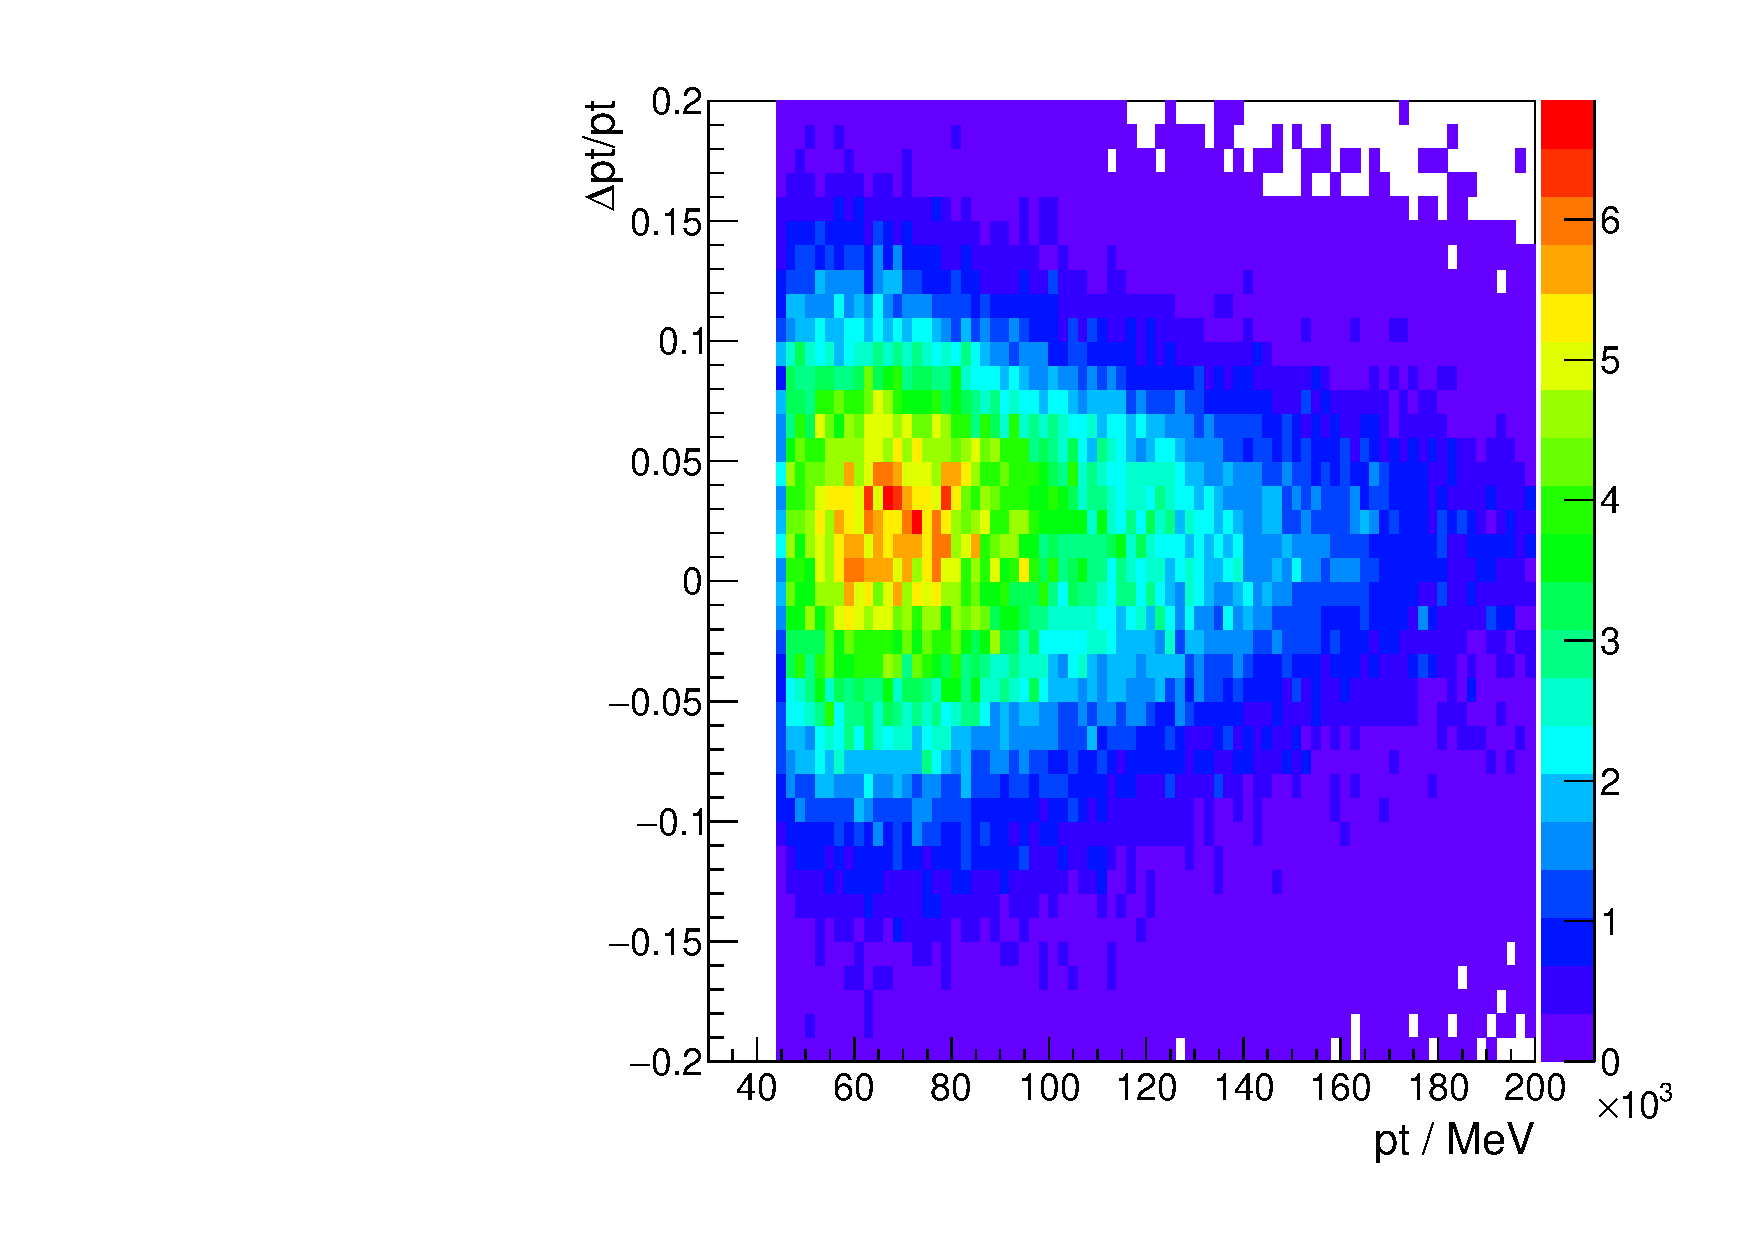
\includegraphics[width=1\linewidth]{ptRatio_Leading_BJet}

			\end{minipage}
			\quad
			\begin{minipage}[h]{0.33\linewidth}
				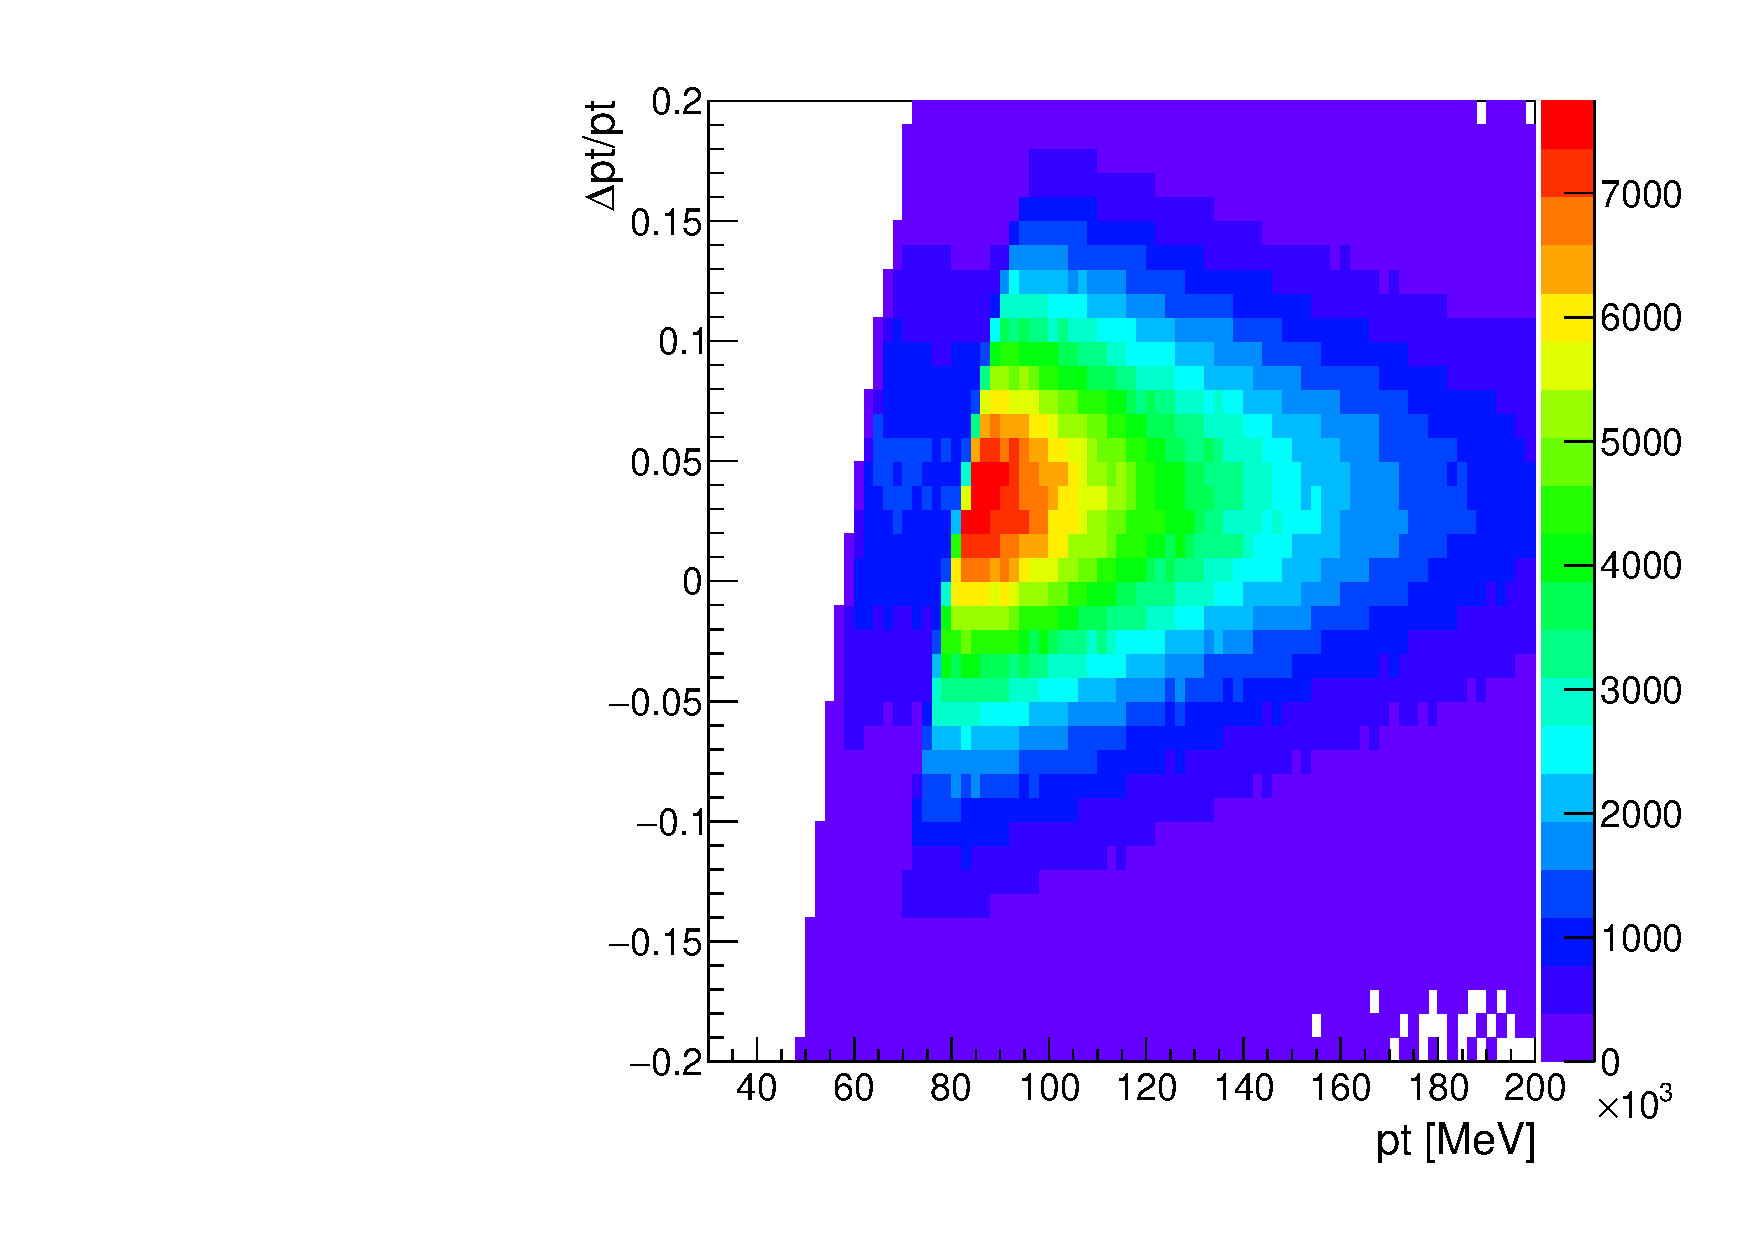
\includegraphics[width=1\linewidth]{Offline_2C_ptRatio_Leading_BJet}
			\end{minipage}
			\caption{$\Delta $\pt$_{ratio}$ for the leading \pt $b$-jet against \pt of the offline $b$-jet, plotted for Monte-Carlo simulated results (left) and real data (right).}
			\label{fig:O:leadingbpt}
		\end{figure}
		
		The comparative performance of the online and offline jets is \pt is broadly similar for events in both Data and Monte-Carlo. The bulk of the results occur with a $\Delta$\pt$_{ratio}\sim0$ and the two plots show a comparable drop off in \pt distribution. The distinctive curve present in the results from the Data is an artefact of the trigger used in real data, which is not required for the Monte-Carlo. As discussed in \todo{make this point}, the real Data was required to pass a trigger with at least one jet with a \pt$>80$GeV which results in the steep drop-off below this cut value. 
		
		The distribution of the $\Delta$\pt$_{ratio}$ about 0 can be shown by taking a slice across the distribution for a representative \pt value. The $\Delta $\pt$_{ratio}$ values wer also split into $\eta$ bands to study performance at different points in the detector. For the leading \bjet, this is constrained to be within the region of the detector (Section \ref{D:btagging}) where \btagging is available.   
		
		\begin{figure}[h]
			\centering

			\begin{minipage}[h]{0.33\linewidth}
				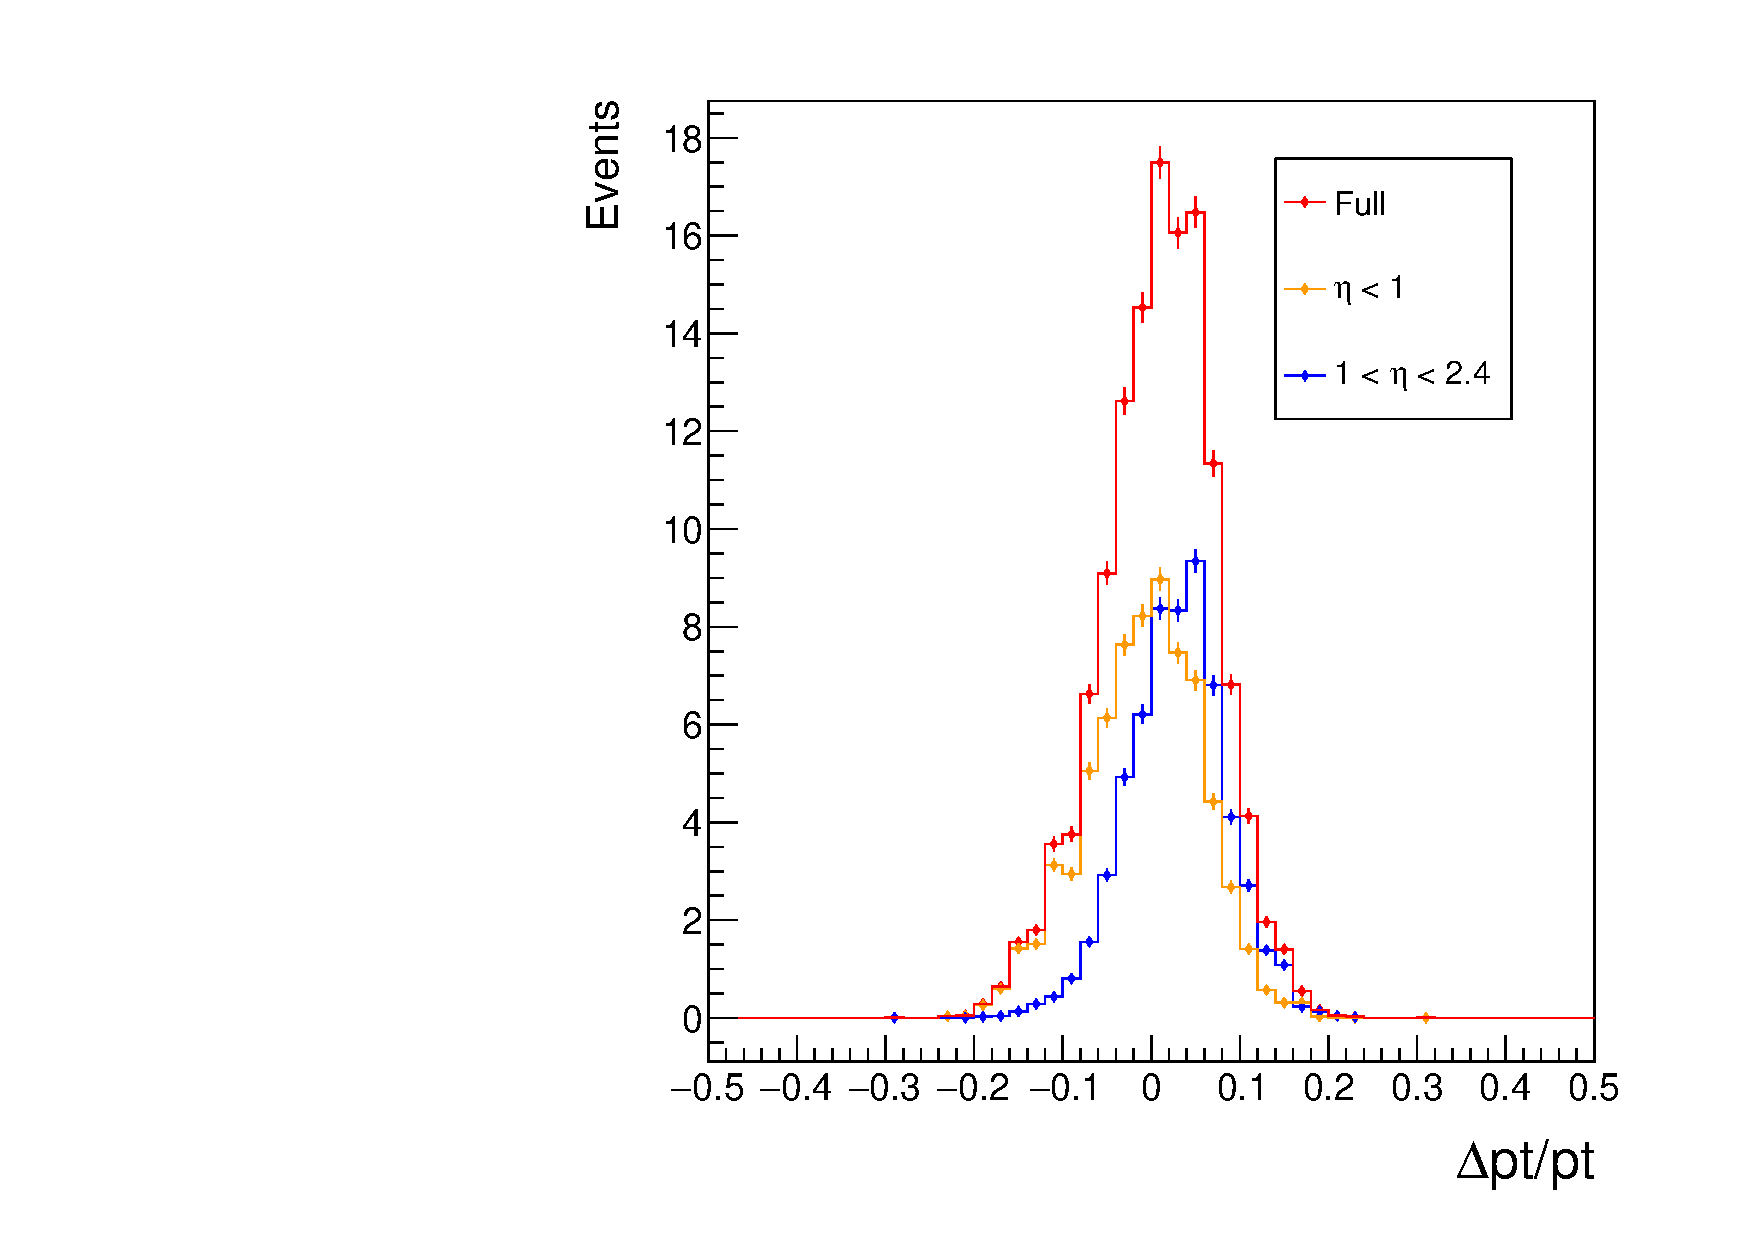
\includegraphics[width=1\linewidth]{Slices_ptRatio_Leading_BJet}
			\end{minipage}
			\quad
			\begin{minipage}[h]{0.33\linewidth}
				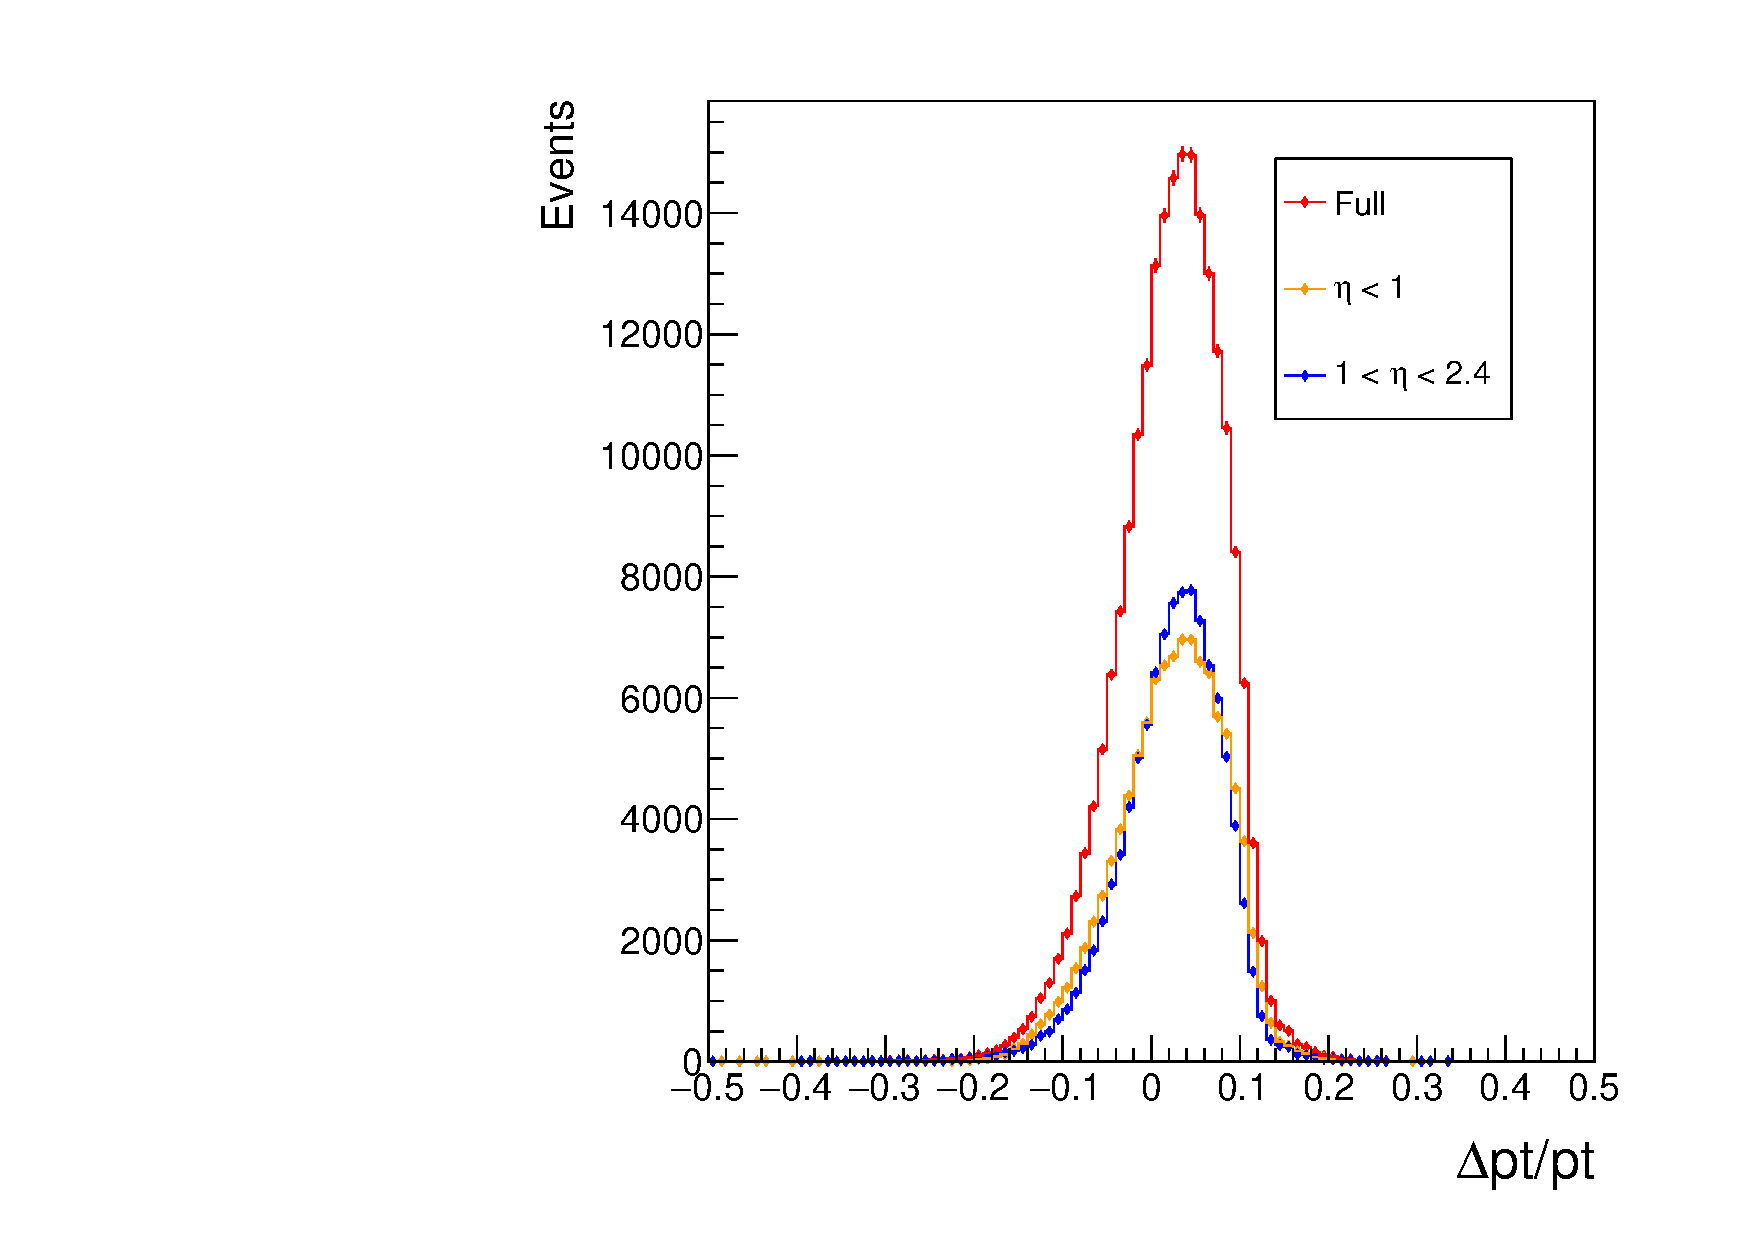
\includegraphics[width=1\linewidth]{Slices_Data_ptRatio_Leading_BJet}
			\end{minipage}
			\caption{$\Delta $\pt$_{ratio}$ distribution for the leading \bjet with $89<$\pt$<91$ GeV. The distributions for all events and events split by $\eta$ region are shown.}
			\label{fig:O:leadingbptslice}
		\end{figure}
		
		 The results show similar profiles between the Monte-Carlo and Data events for $\Delta$\pt$_{ratio}$. Both plots show the offline \pt values to be consitantly higher than the online, with a median shift of $4\%$ in Data and $2\%$ in Monte-Carlo. The performance between $\eta$ ranges was also consistent. The profiles broadly match the full shape and each other, but the Monte-Carlo showed a slight difference in  $\Delta$\pt$_{ratio}$ value as the central $\eta$ range peaked at $\sim0$. The breadth of these distributions is quite large, with both Data and Monte-Carlo showing $\pm10\%$ in $\Delta$\pt$_{ratio}$.
		
		These comparisons can be carried out for other jet properties (e.g. $\eta$, $\phi$) to confirm the offline and online jets are behaving in a similar fashion.
		
		\begin{figure}[h]
			\centering
			\begin{minipage}[h]{0.33\linewidth}
				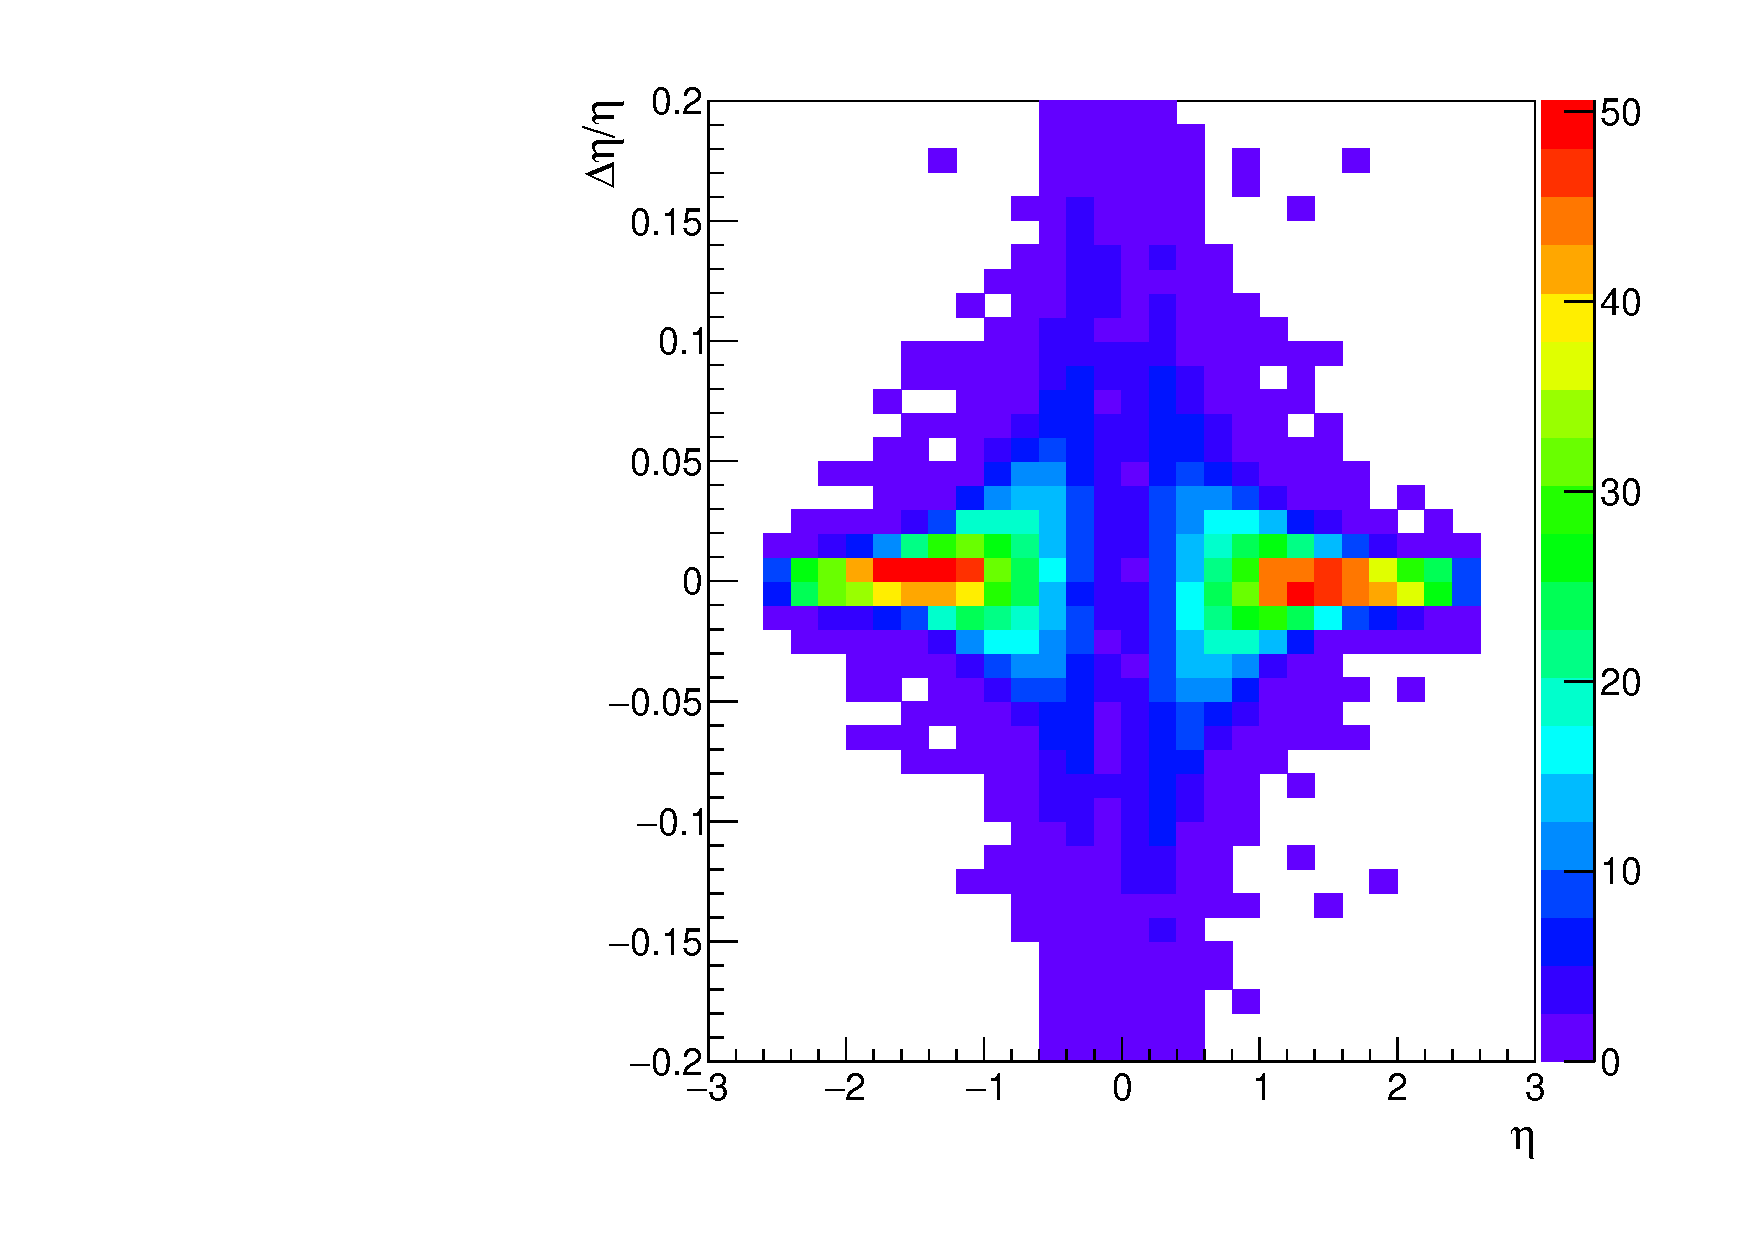
\includegraphics[width=1\linewidth]{etaRatio_Leading_BJet}
				
			\end{minipage}
			\quad
			\begin{minipage}[h]{0.33\linewidth}
				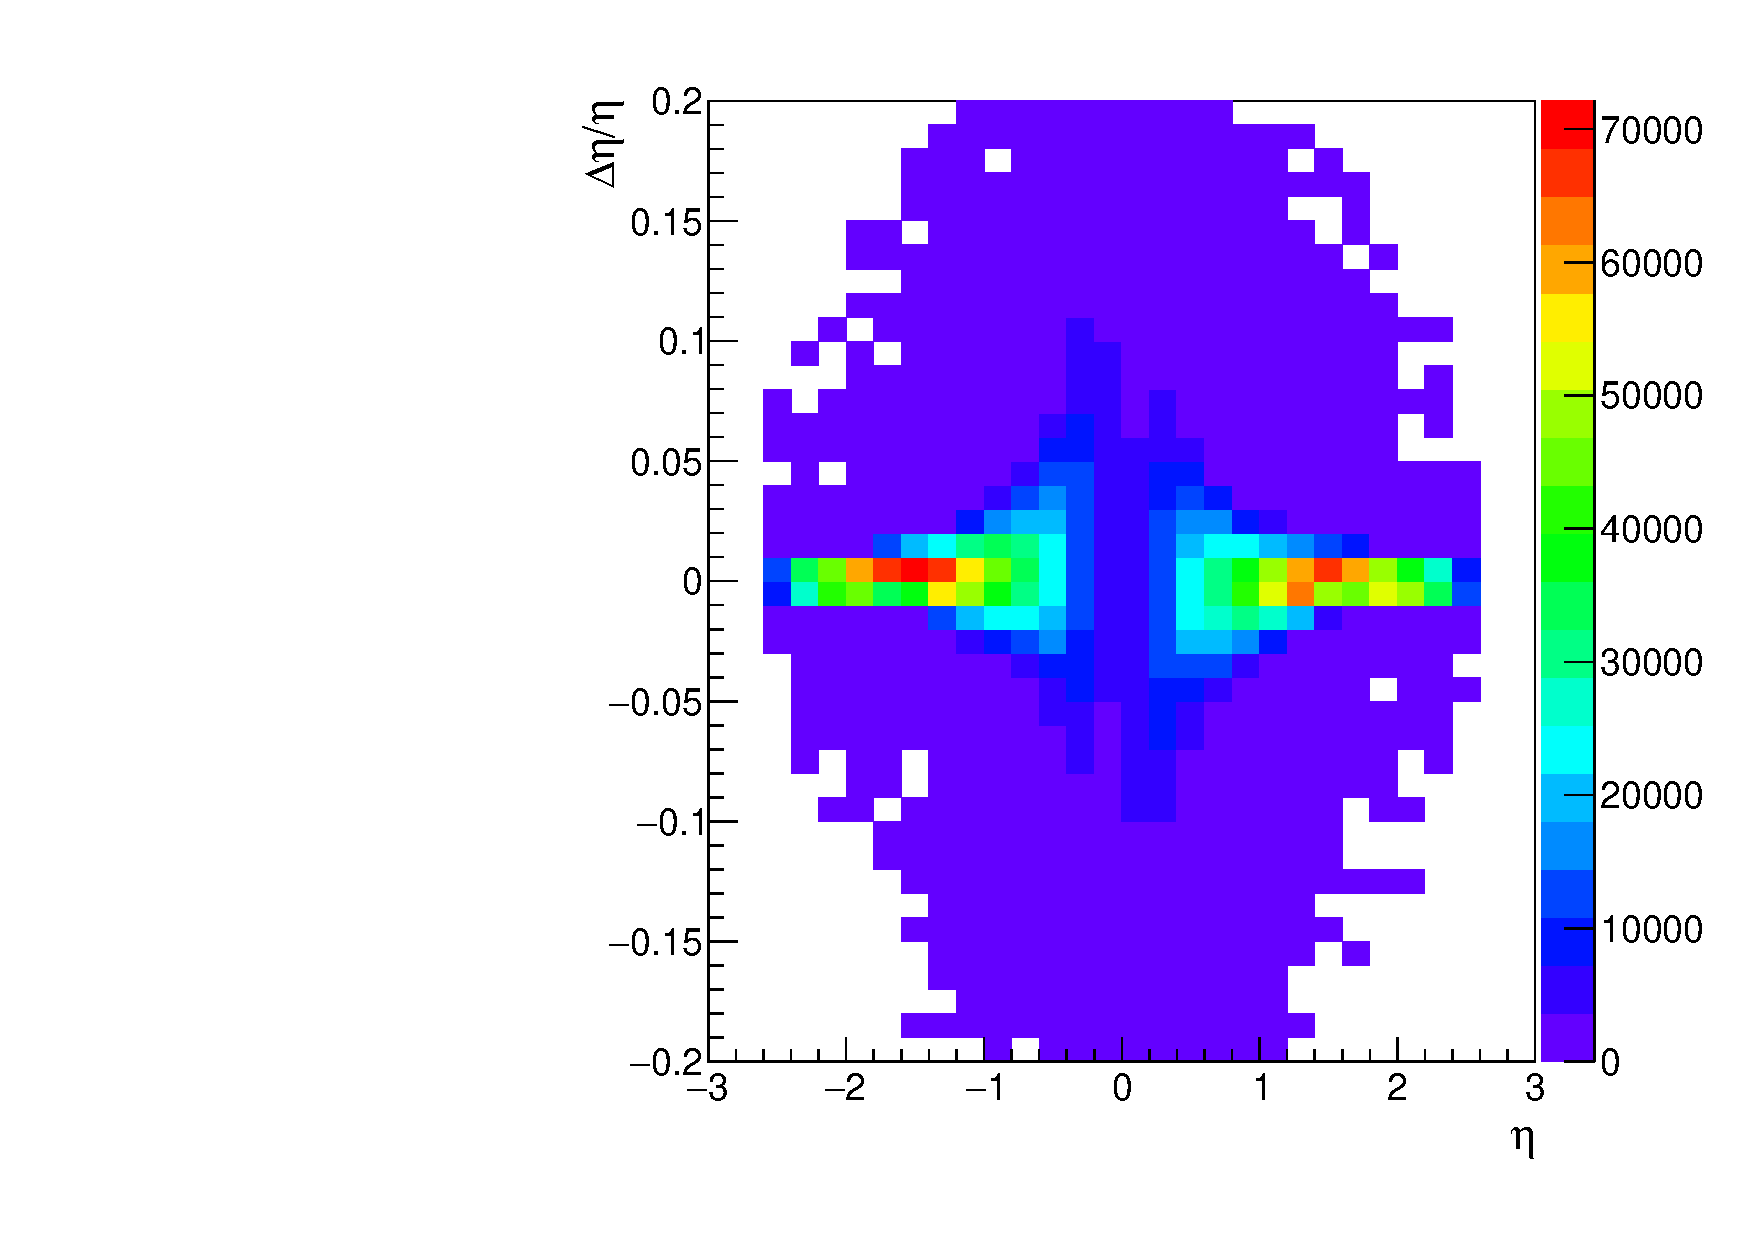
\includegraphics[width=1\linewidth]{Offline_2C_etaRatio_Leading_BJet}
			\end{minipage}
			\caption{$\Delta \eta_{ratio}$ for the leading \bjet, for Monte-Carlo events (left) and real data (right).}
			\label{fig:O:leadingbeta}
		\end{figure}
		
		\begin{figure}[h]
			\centering
			\begin{minipage}[h]{0.33\linewidth}
				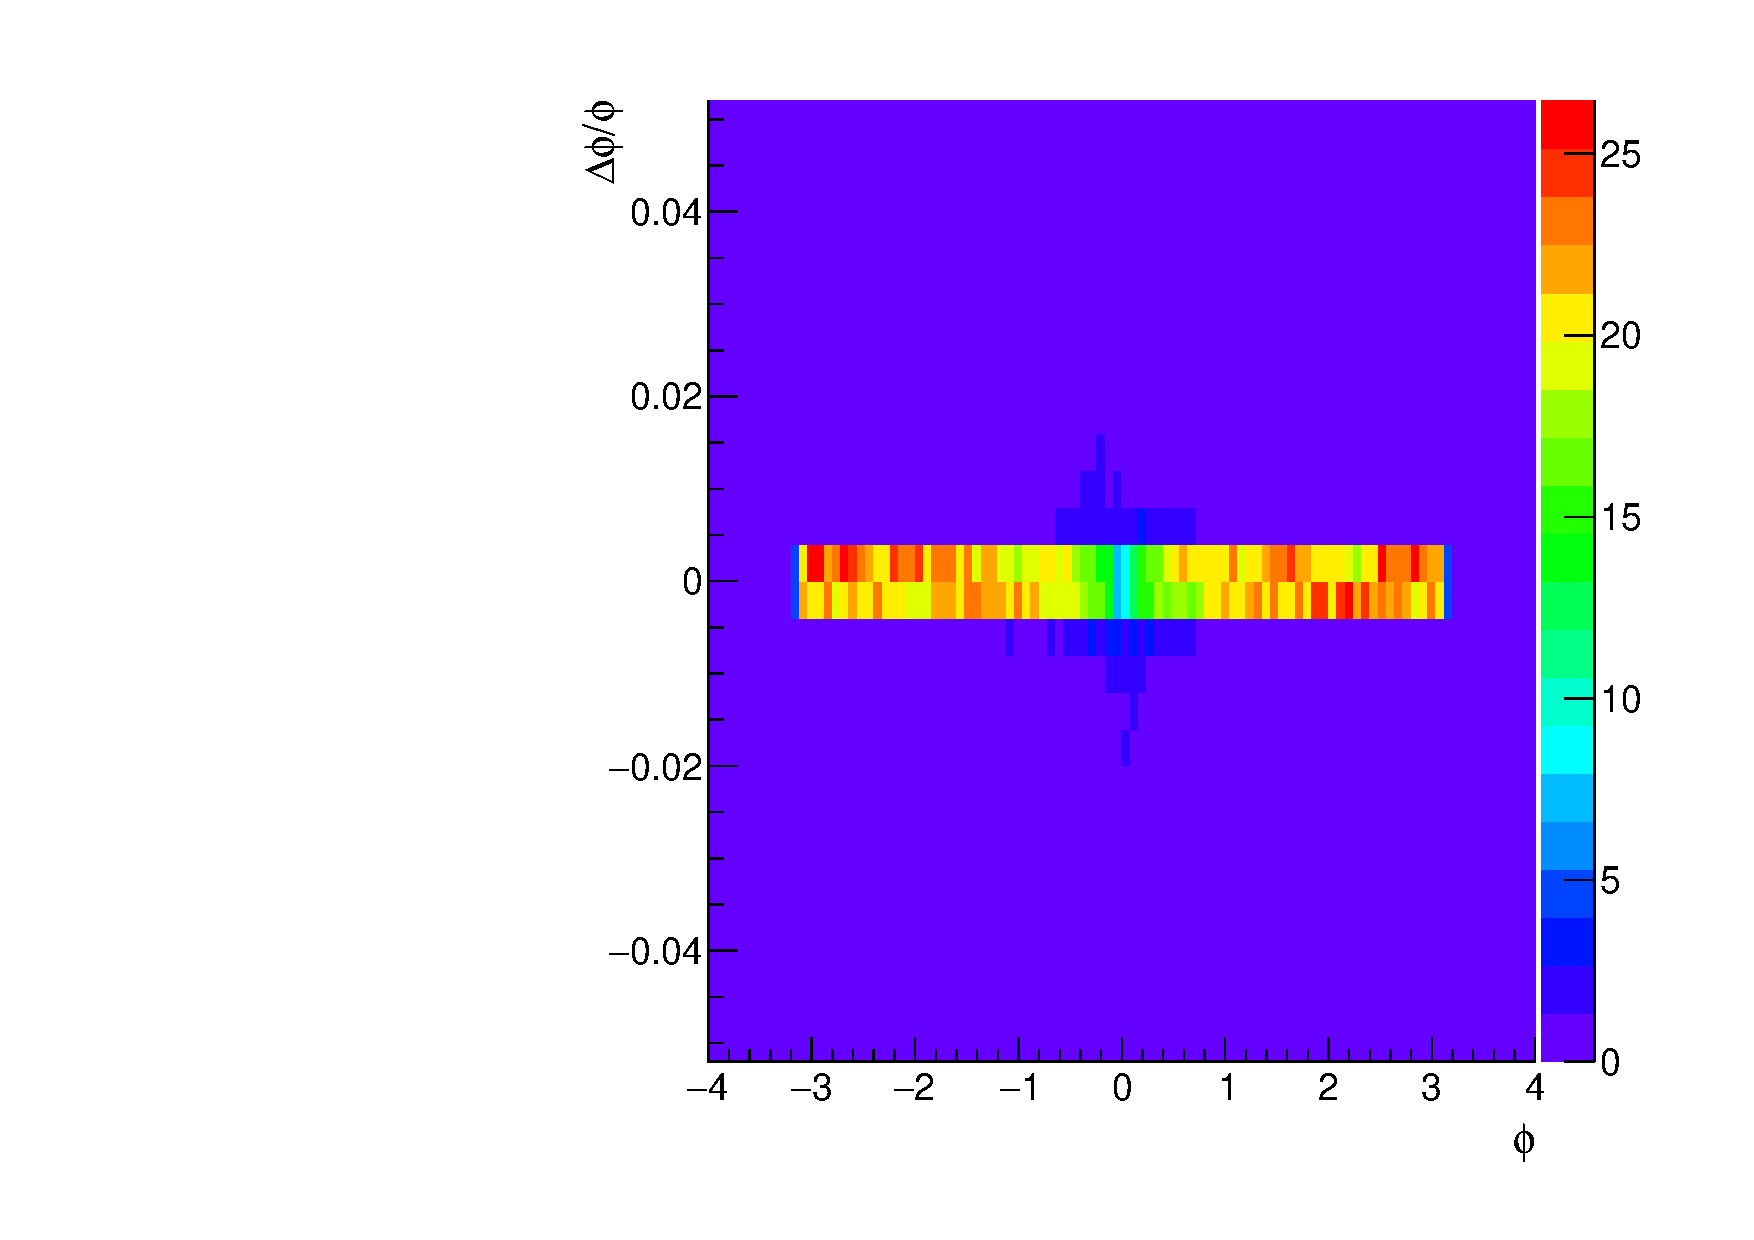
\includegraphics[width=1\linewidth]{phiRatio_Leading_BJet}
				
			\end{minipage}
			\quad
			\begin{minipage}[h]{0.33\linewidth}
				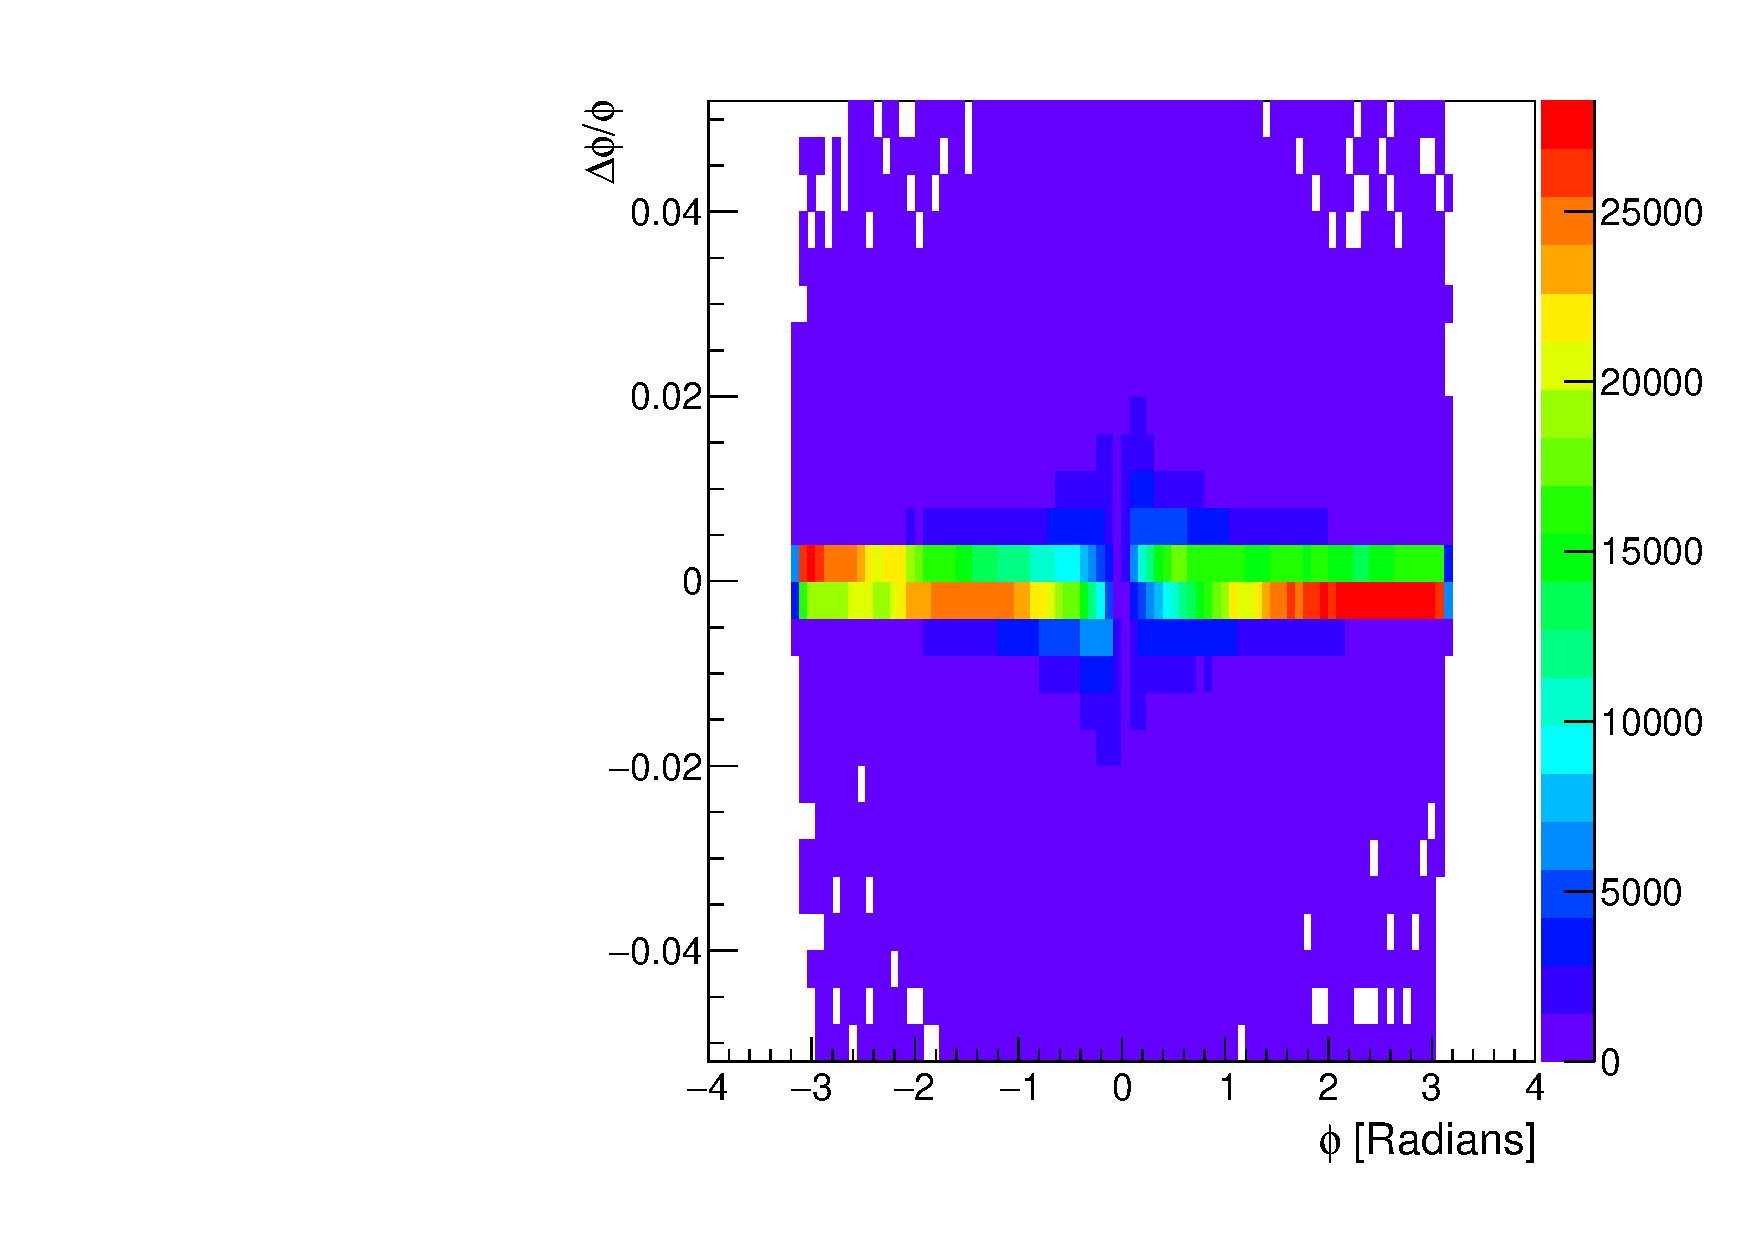
\includegraphics[width=1\linewidth]{Offline_2C_phiRatio_Leading_BJet}
			\end{minipage}
			\caption{$\Delta \phi_{ratio}$for the leading \bjet, for Monte-Carlo events (left) and real data (right).}
			\label{fig:O:leadingbphi}
		\end{figure}
		
		The Data and Monte-Carlo distributions for these values are extermely similar to each other, and also show very close agreement between the values for offline and online jet objects. In both cases the median $\Delta X_{ratio}$ value is $\sim0$ and the breadth of the distribution is less than $1\%$ of the value. 
		

\newpage
\section{Leading Non \textit{b}-jets}
	\label{OP:leadingnonb}
	
	For \VBFHBB the pair of high \pt forward jets is the other significant feature, so the offline/online performance in the leading Non \bjet was studied.
	
	\todo{Do we require this to fail the btagging}
	
	\begin{figure}[h]
		\centering
		\begin{minipage}[h]{0.33\linewidth}
			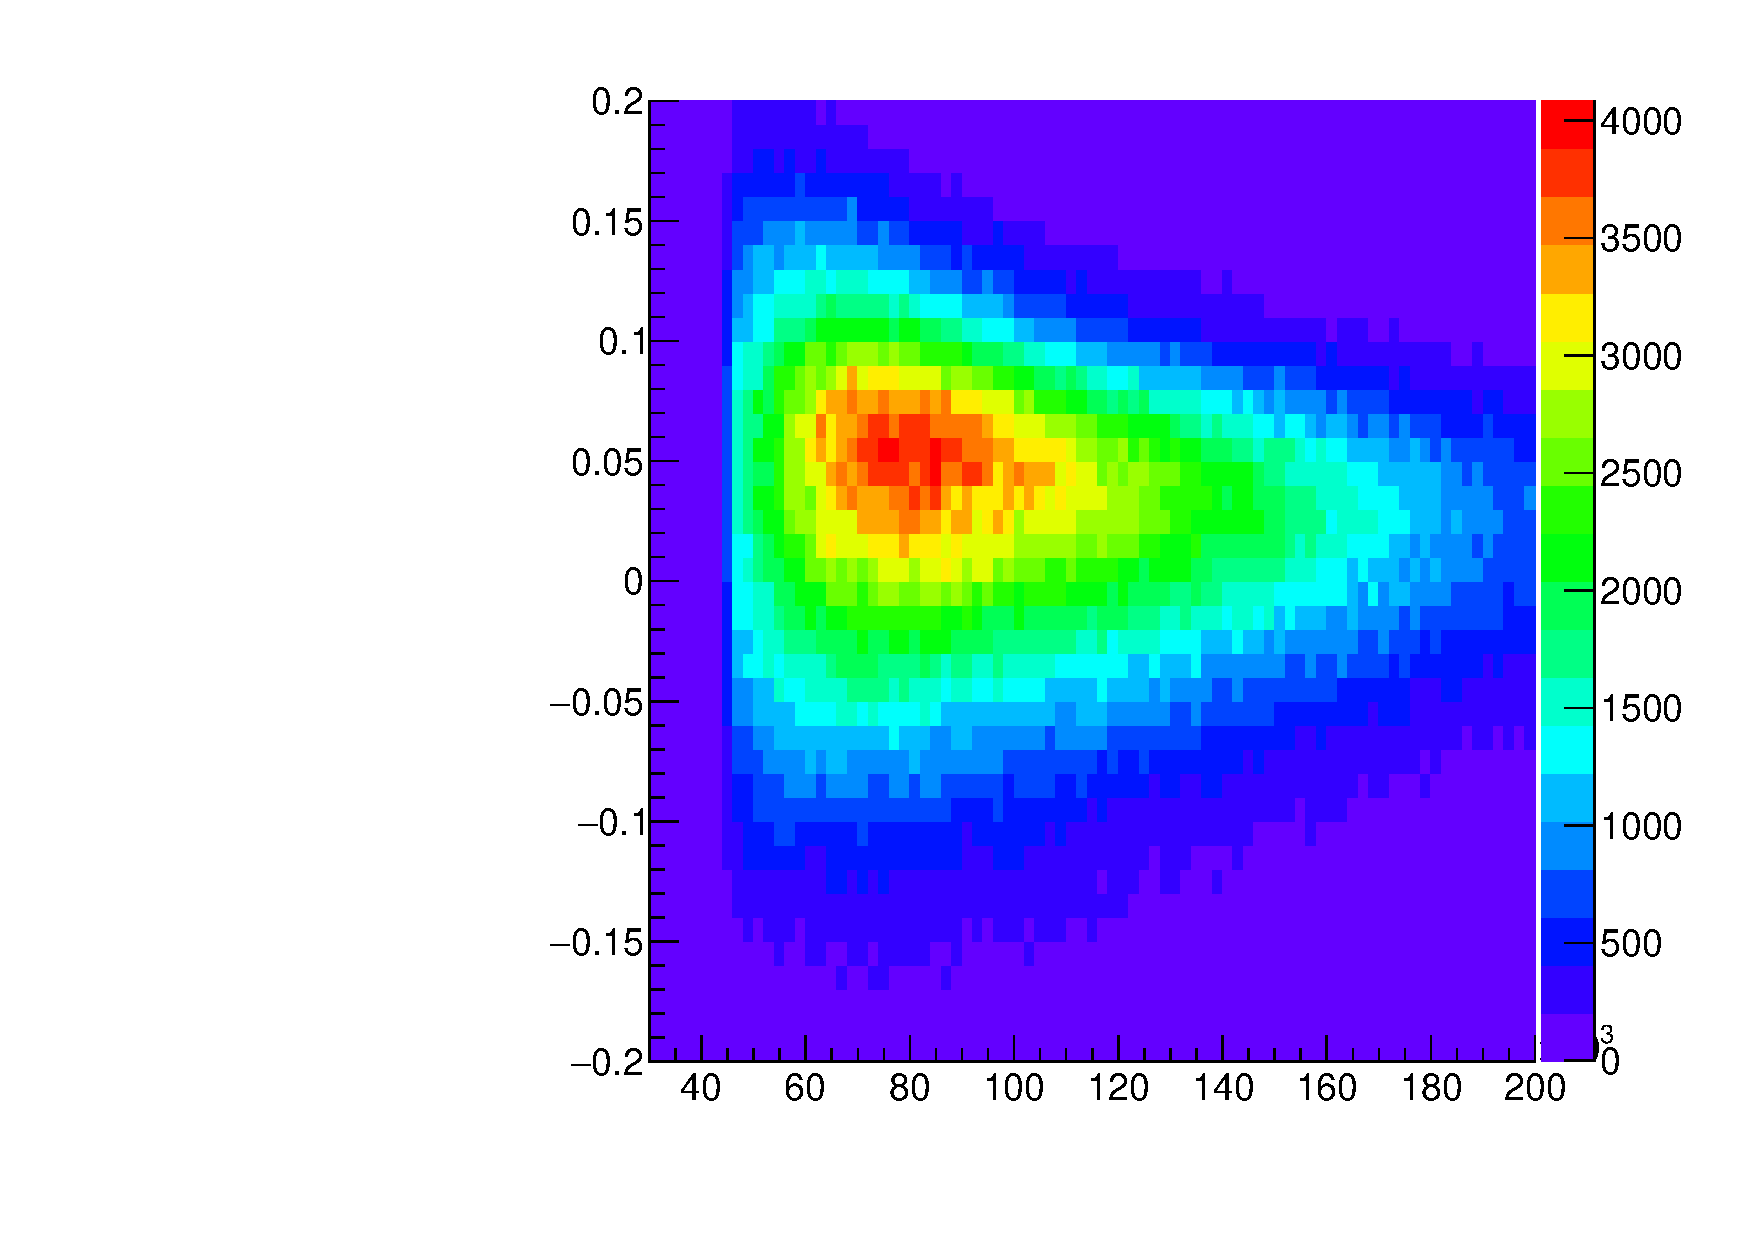
\includegraphics[width=1\linewidth]{ptRatio_Leading_Non_BJet}
			
		\end{minipage}
		\quad
		\begin{minipage}[h]{0.33\linewidth}
			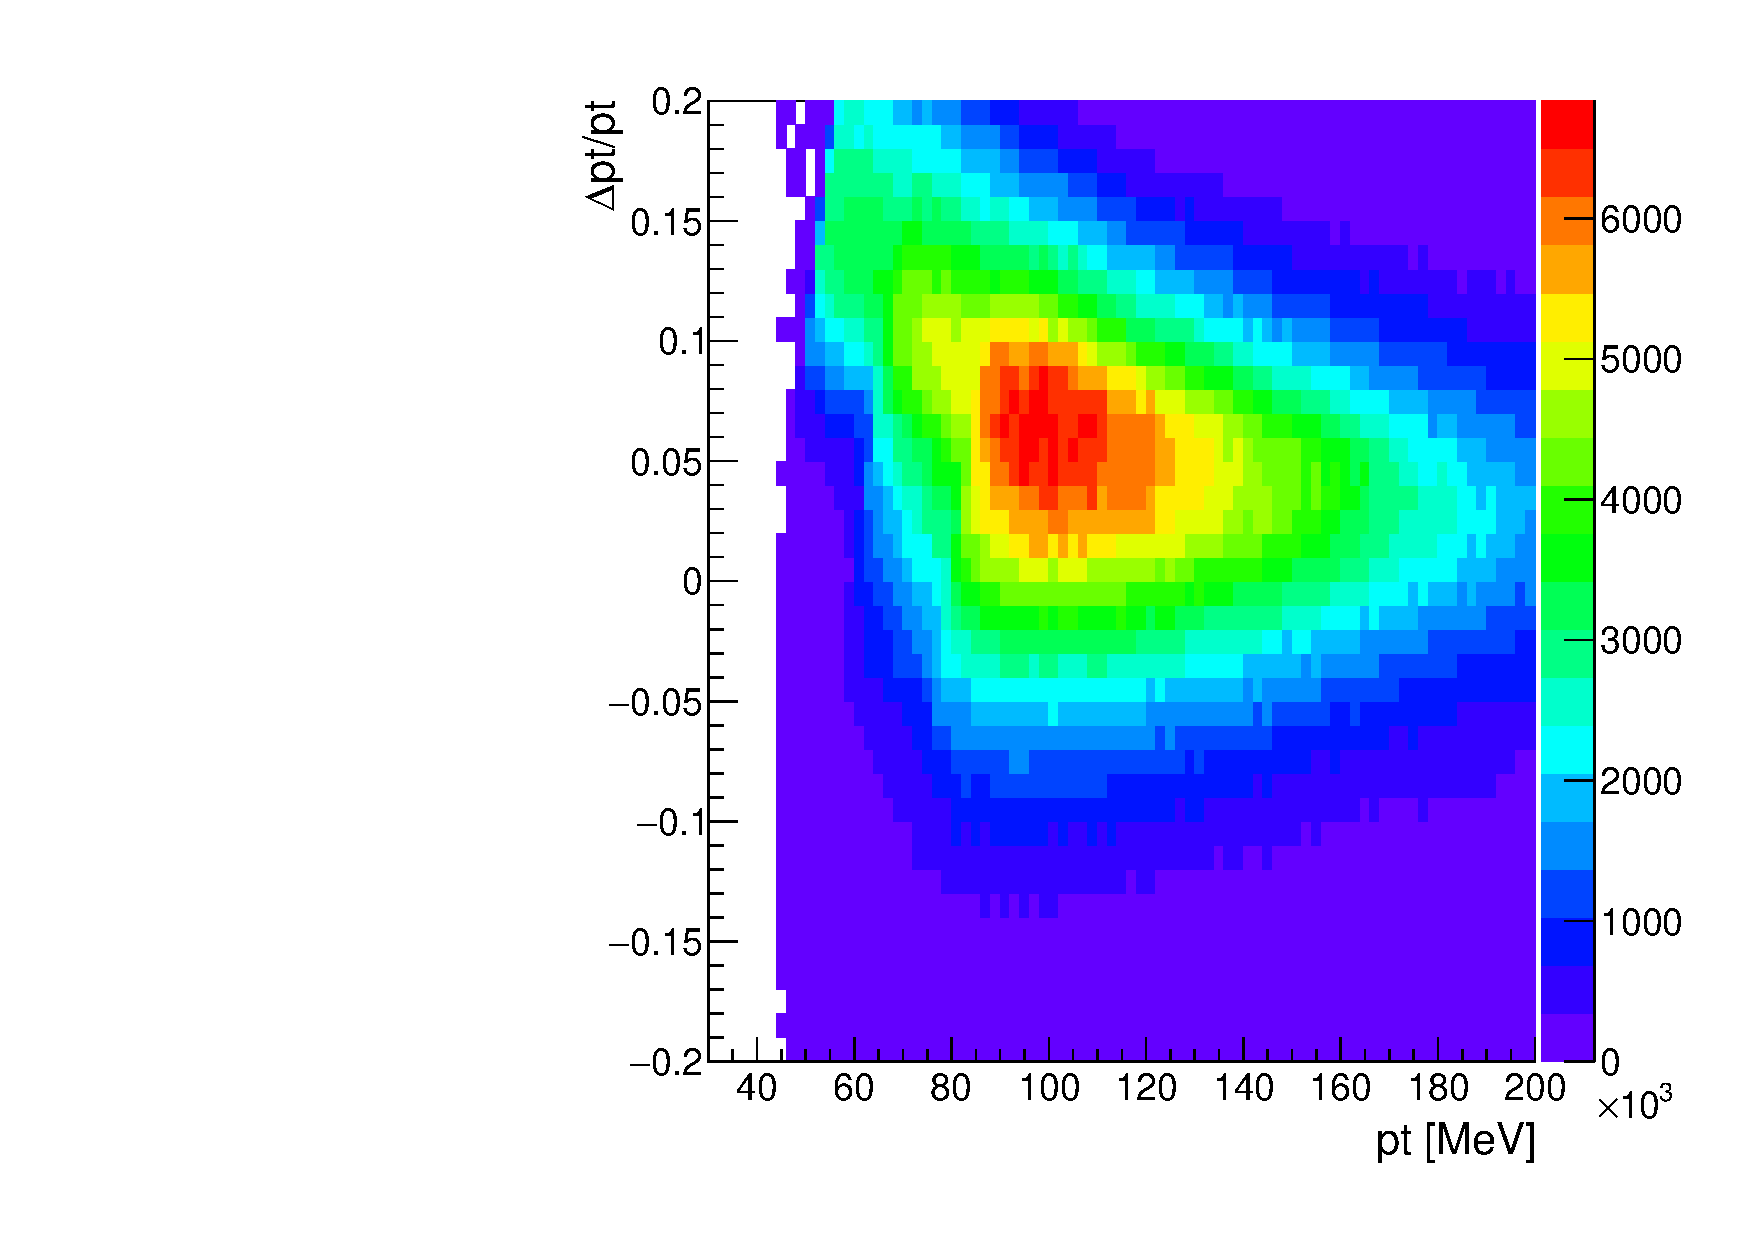
\includegraphics[width=1\linewidth]{Offline_2C_ptRatio_Leading_Non_BJet}
		\end{minipage}
		\caption{$\Delta $\pt$_{ratio}$ for the leading \pt non $b$-jet against \pt of the offline jet, plotted for Monte-Carlo simulated results (left) and real data (right).}
		\label{fig:O:leadingnonbpt}
	\end{figure}
	
	The leading non \bjet shows a similar situation to the leading \bjet. At the peak of the $\Delta $\pt$_{ratio}$ distribution the \pt of the offline jet is within $5\%$ of the online \pt, and the overall shape of the distribution is comparable between the Monte-Carlo and real Data events. As with the \bjets, the trigger in the real data required a jet in the forward region with \pt$>45$GeV. 
	
	The results could also be split across $\eta$ regions, with the added ability to study the forward regions of the detector. 
	
	\begin{figure}[h]
		\centering
		
		\begin{minipage}[h]{0.33\linewidth}
			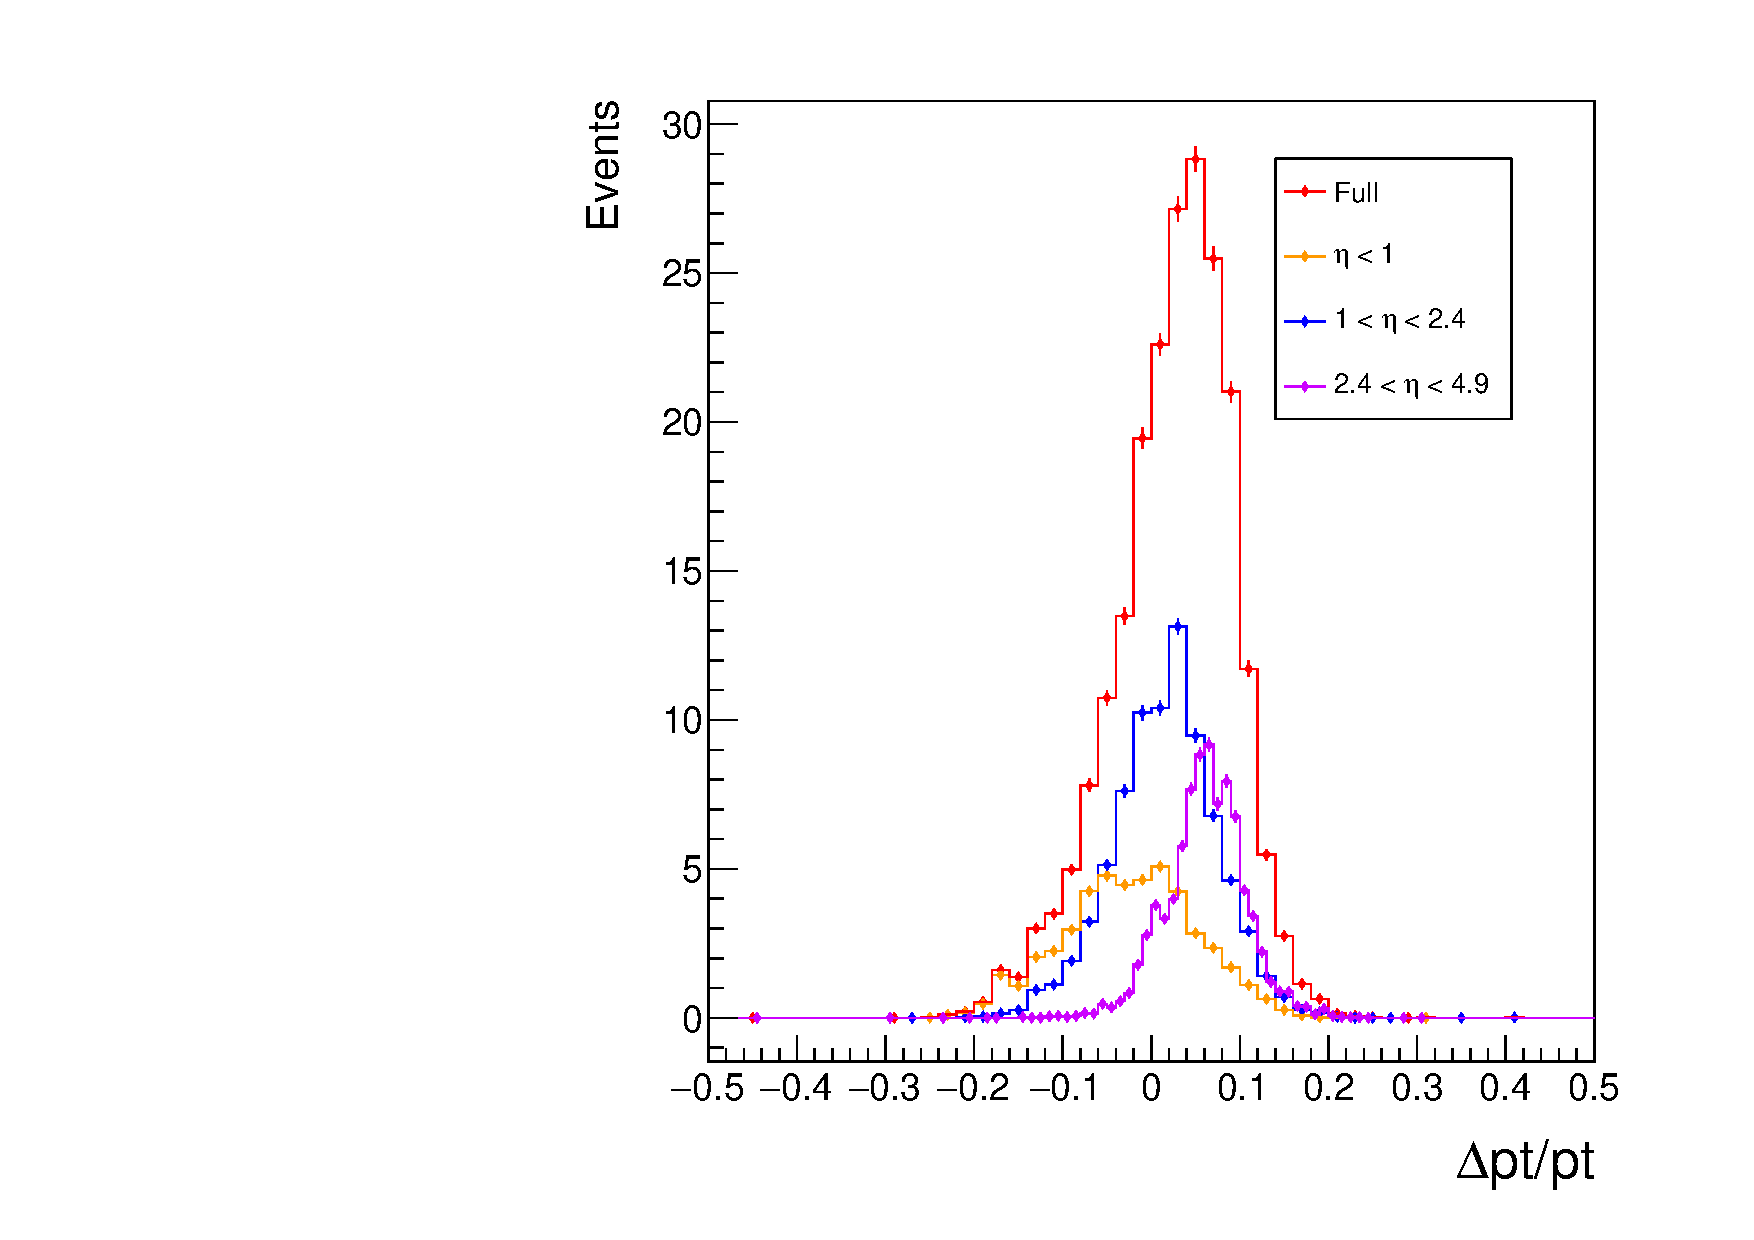
\includegraphics[width=1\linewidth]{Slices_ptRatio_Leading_Non_BJet}
		\end{minipage}
		\quad
		\begin{minipage}[h]{0.33\linewidth}
			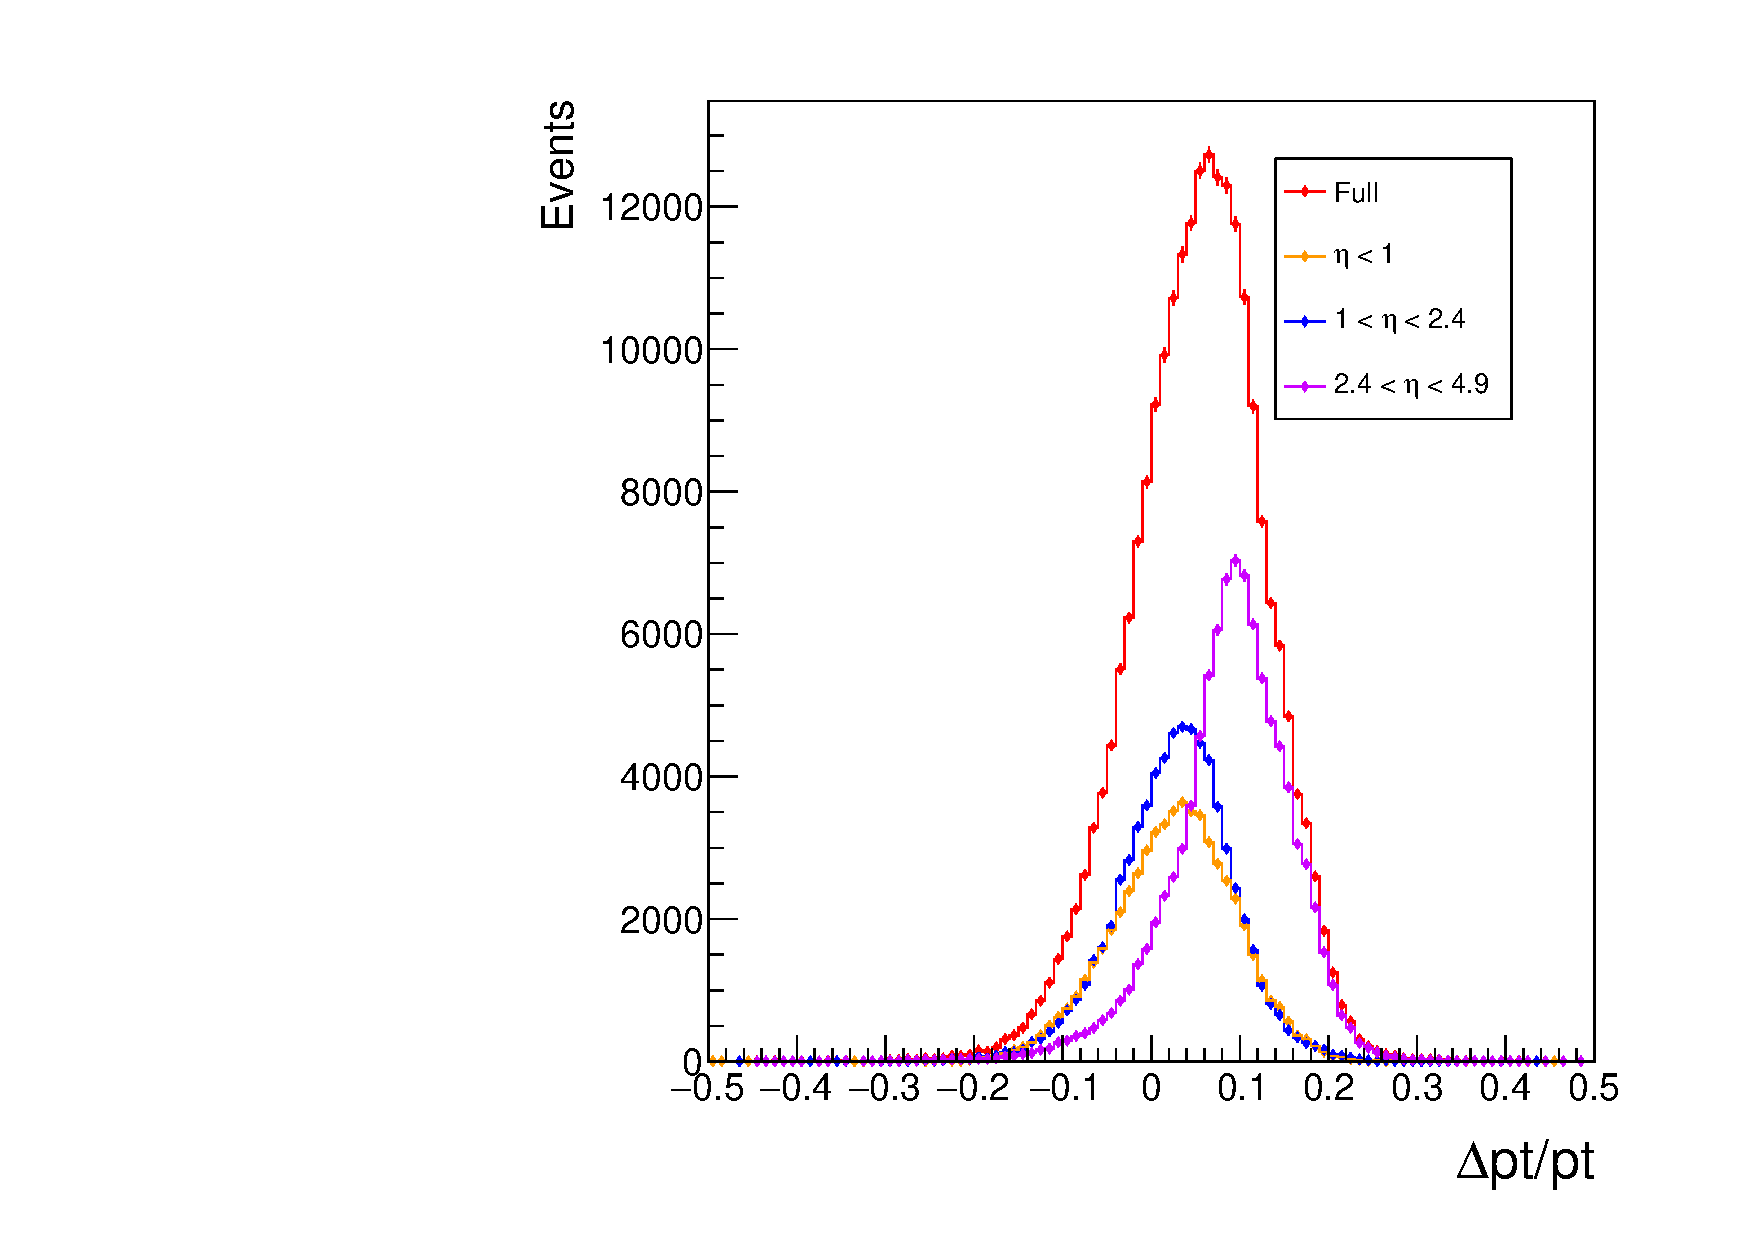
\includegraphics[width=1\linewidth]{Slices_Data_ptRatio_Leading_Non_BJet}
		\end{minipage}
		\caption{$\Delta $\pt$_{ratio}$ distribution for the leading non \bjet with $89<$\pt$<91$ GeV. The distributions for all events and events split by $\eta$ region are shown.}
		\label{fig:O:leadingnonbptslice}
	\end{figure}
	
	Both Monte-Carlo and Data show offline jets to be consistently higher \pt than online by $4\%$ and $6\%$ respectively. The overall distribution shape is similar between the simulated and real events, and the shape of the distributions for each $\eta$ band is also comparable. Both the MC and the Data show that the offset in \pt value is worse for the jets in the forward region than in the central regions of the detector, with a significantly higher median $\Delta $\pt$_{ratio}$. 
	
	The other topological variables can also be compared.
	
	\begin{figure}[h]
		\centering
		\begin{minipage}[h]{0.33\linewidth}
			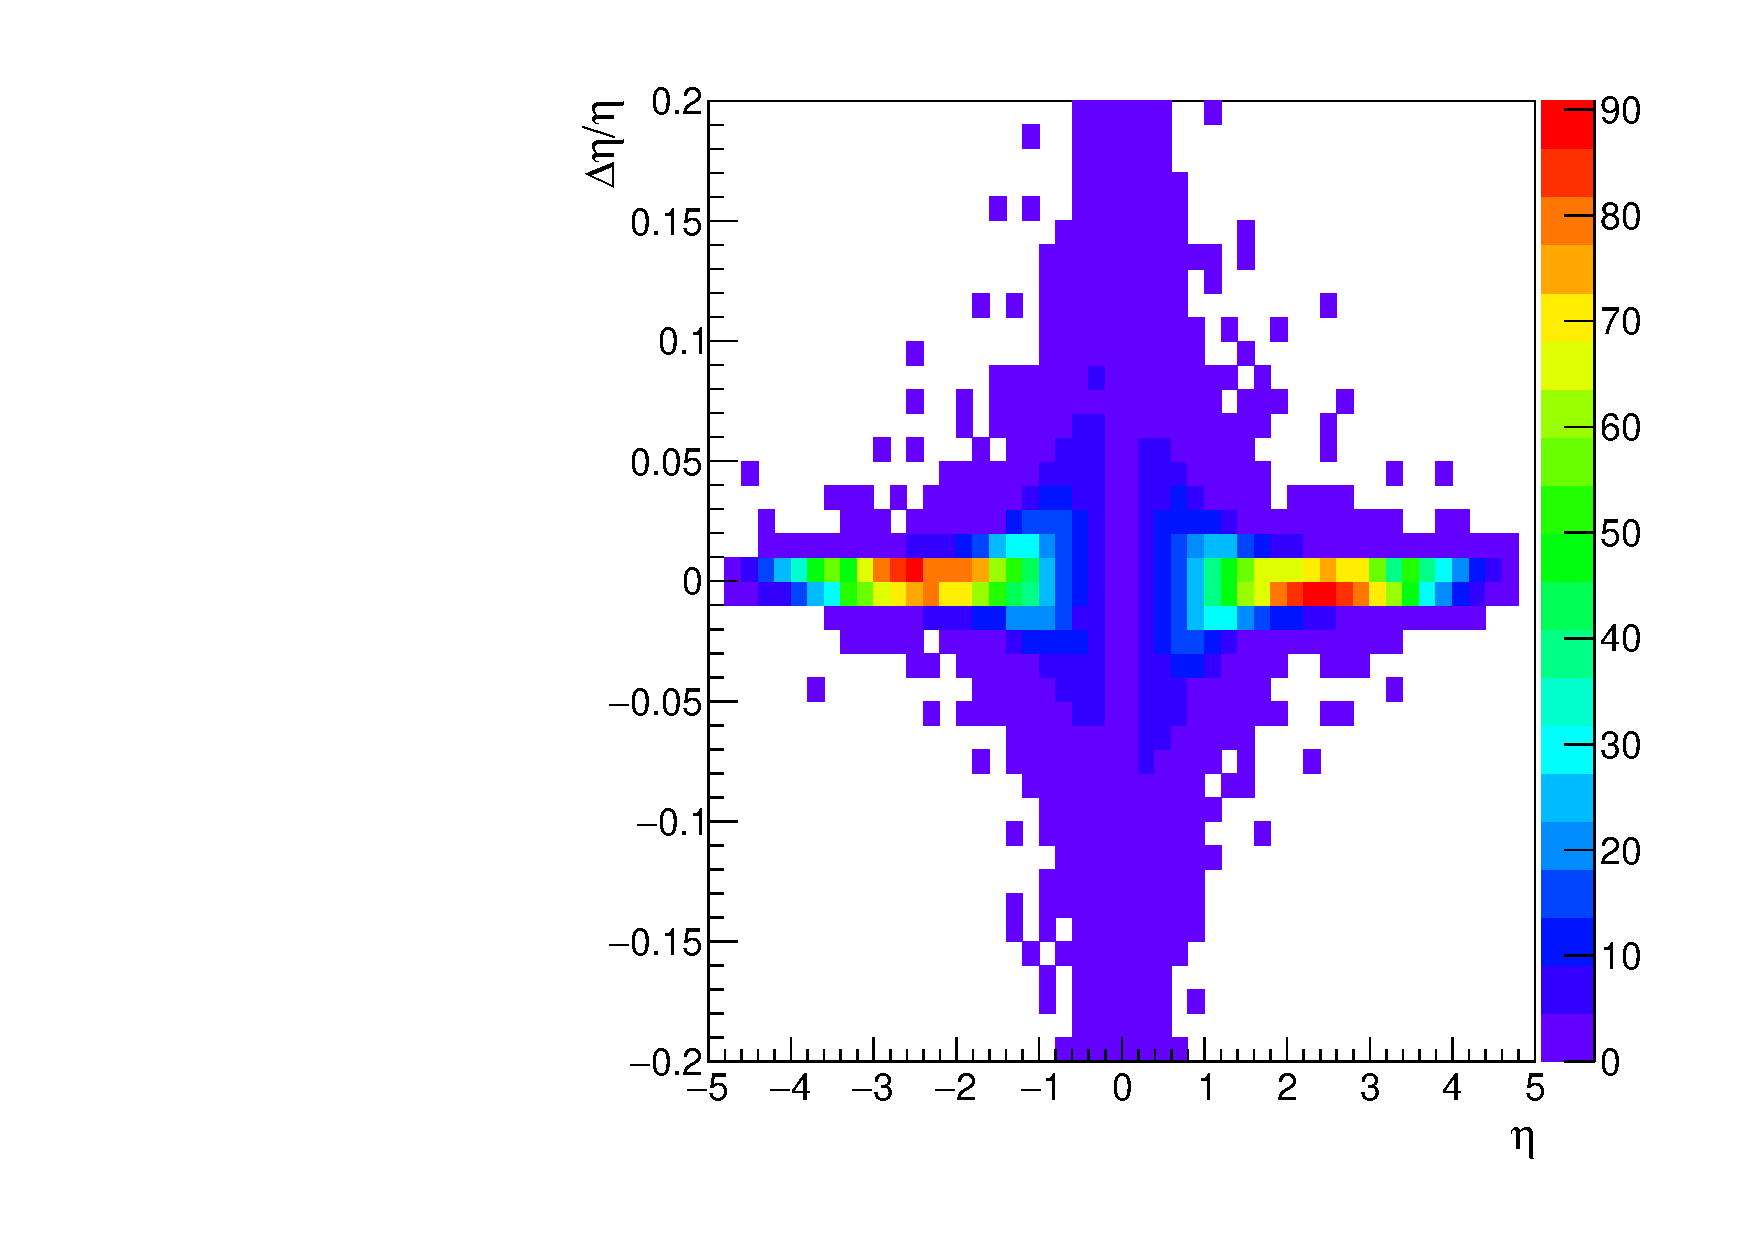
\includegraphics[width=1\linewidth]{etaRatio_Leading_Non_BJet}
			
		\end{minipage}
		\quad
		\begin{minipage}[h]{0.33\linewidth}
			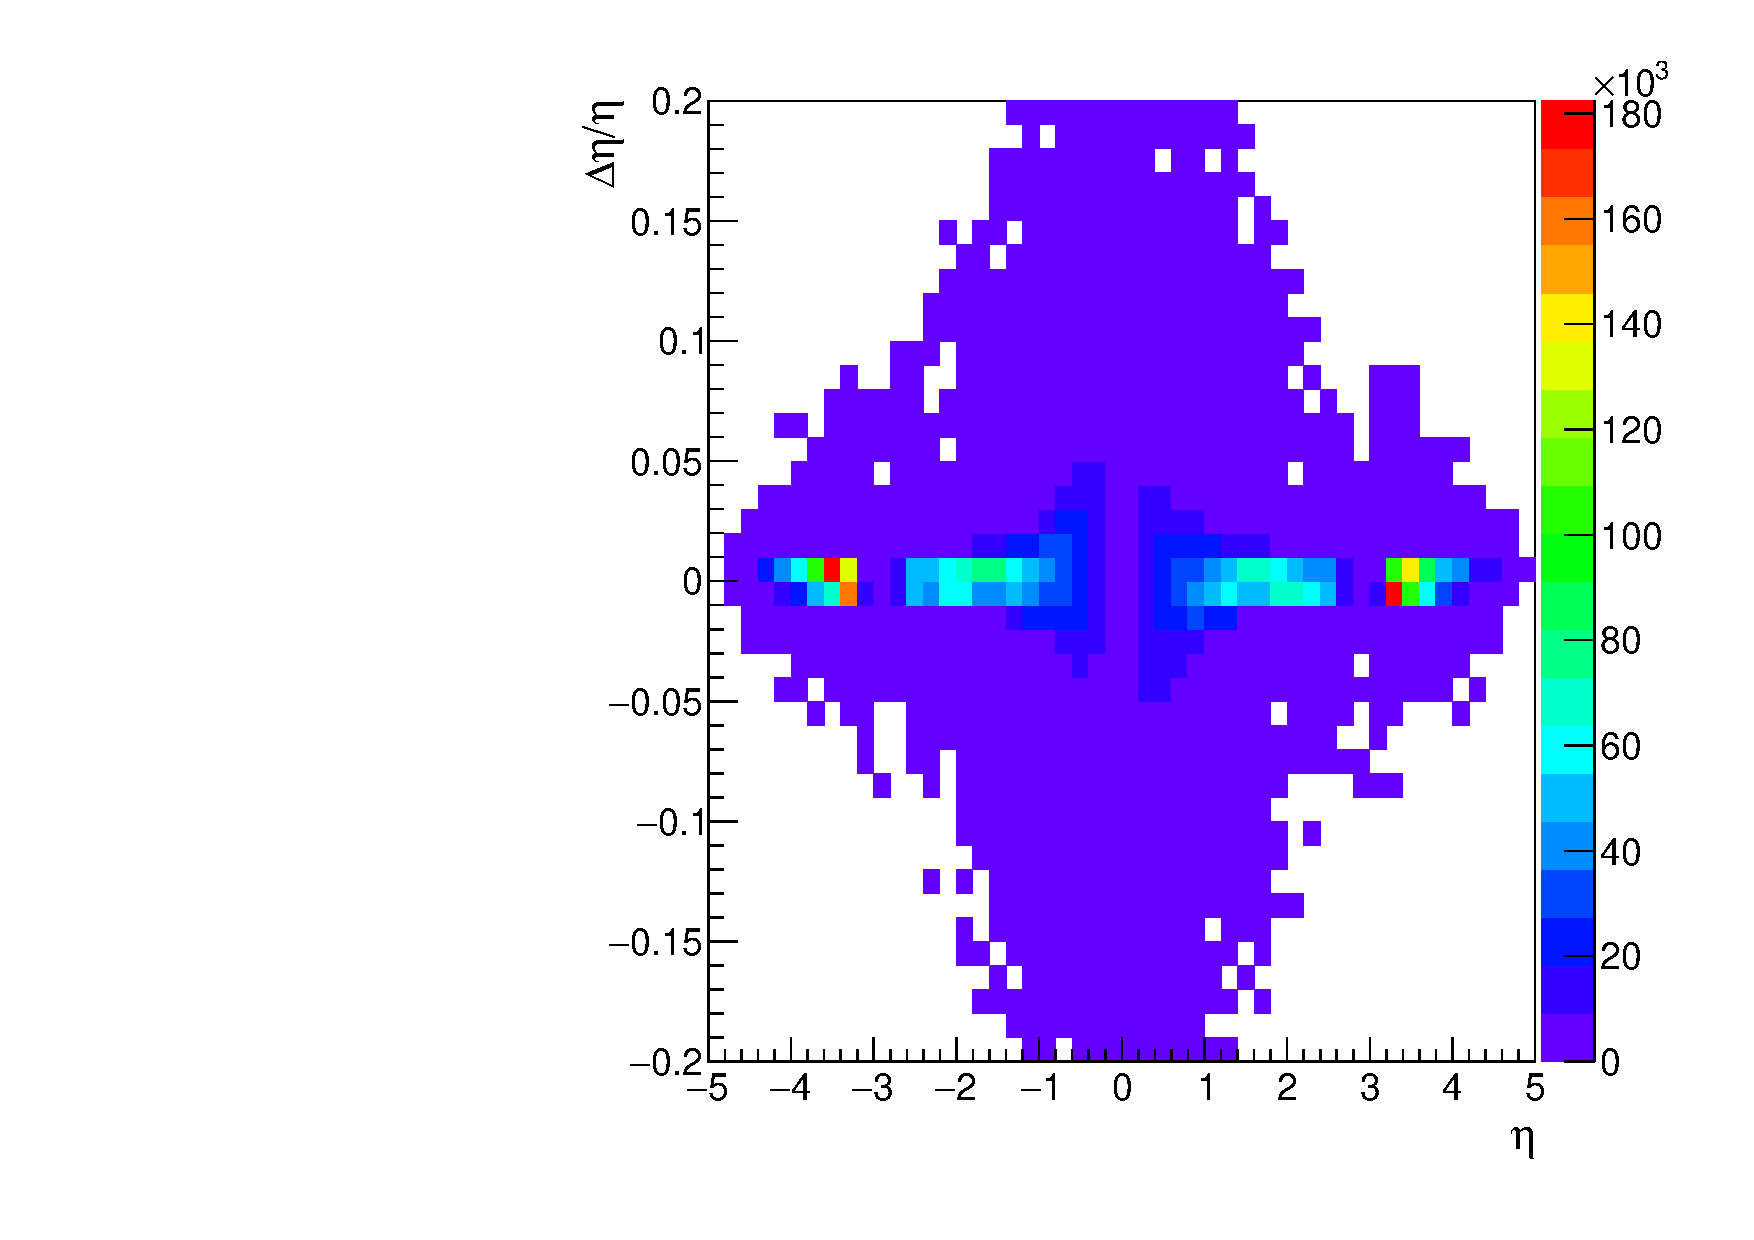
\includegraphics[width=1\linewidth]{Offline_2C_etaRatio_Leading_Non_BJet}
		\end{minipage}
		\caption{$\Delta \eta_{ratio}$ for the leading non \bjet, for Monte-Carlo events (left) and real data (right).}
		\label{fig:O:leadingnonbeta}
	\end{figure}
	
	\begin{figure}[h]
		\centering
		\begin{minipage}[h]{0.33\linewidth}
			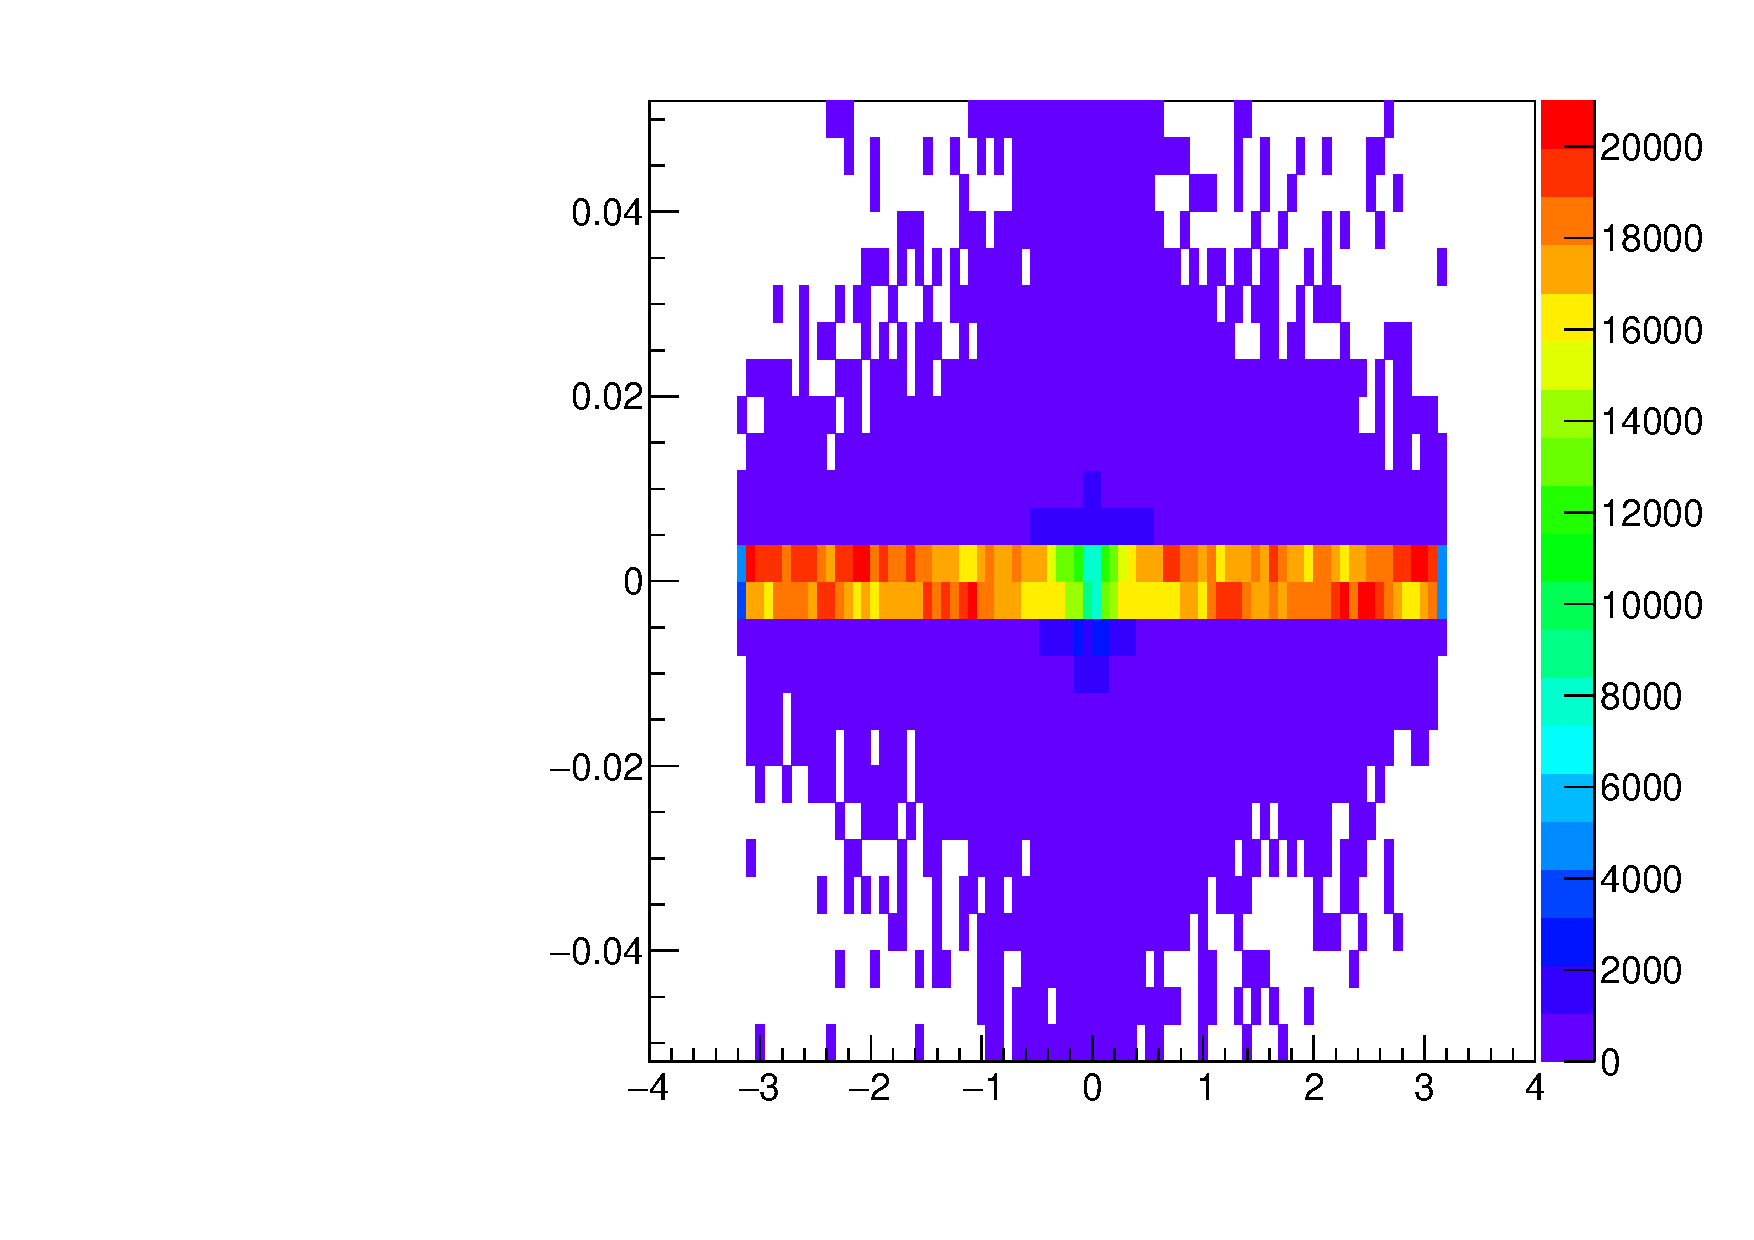
\includegraphics[width=1\linewidth]{phiRatio_Leading_Non_BJet}
			
		\end{minipage}
		\quad
		\begin{minipage}[h]{0.33\linewidth}
			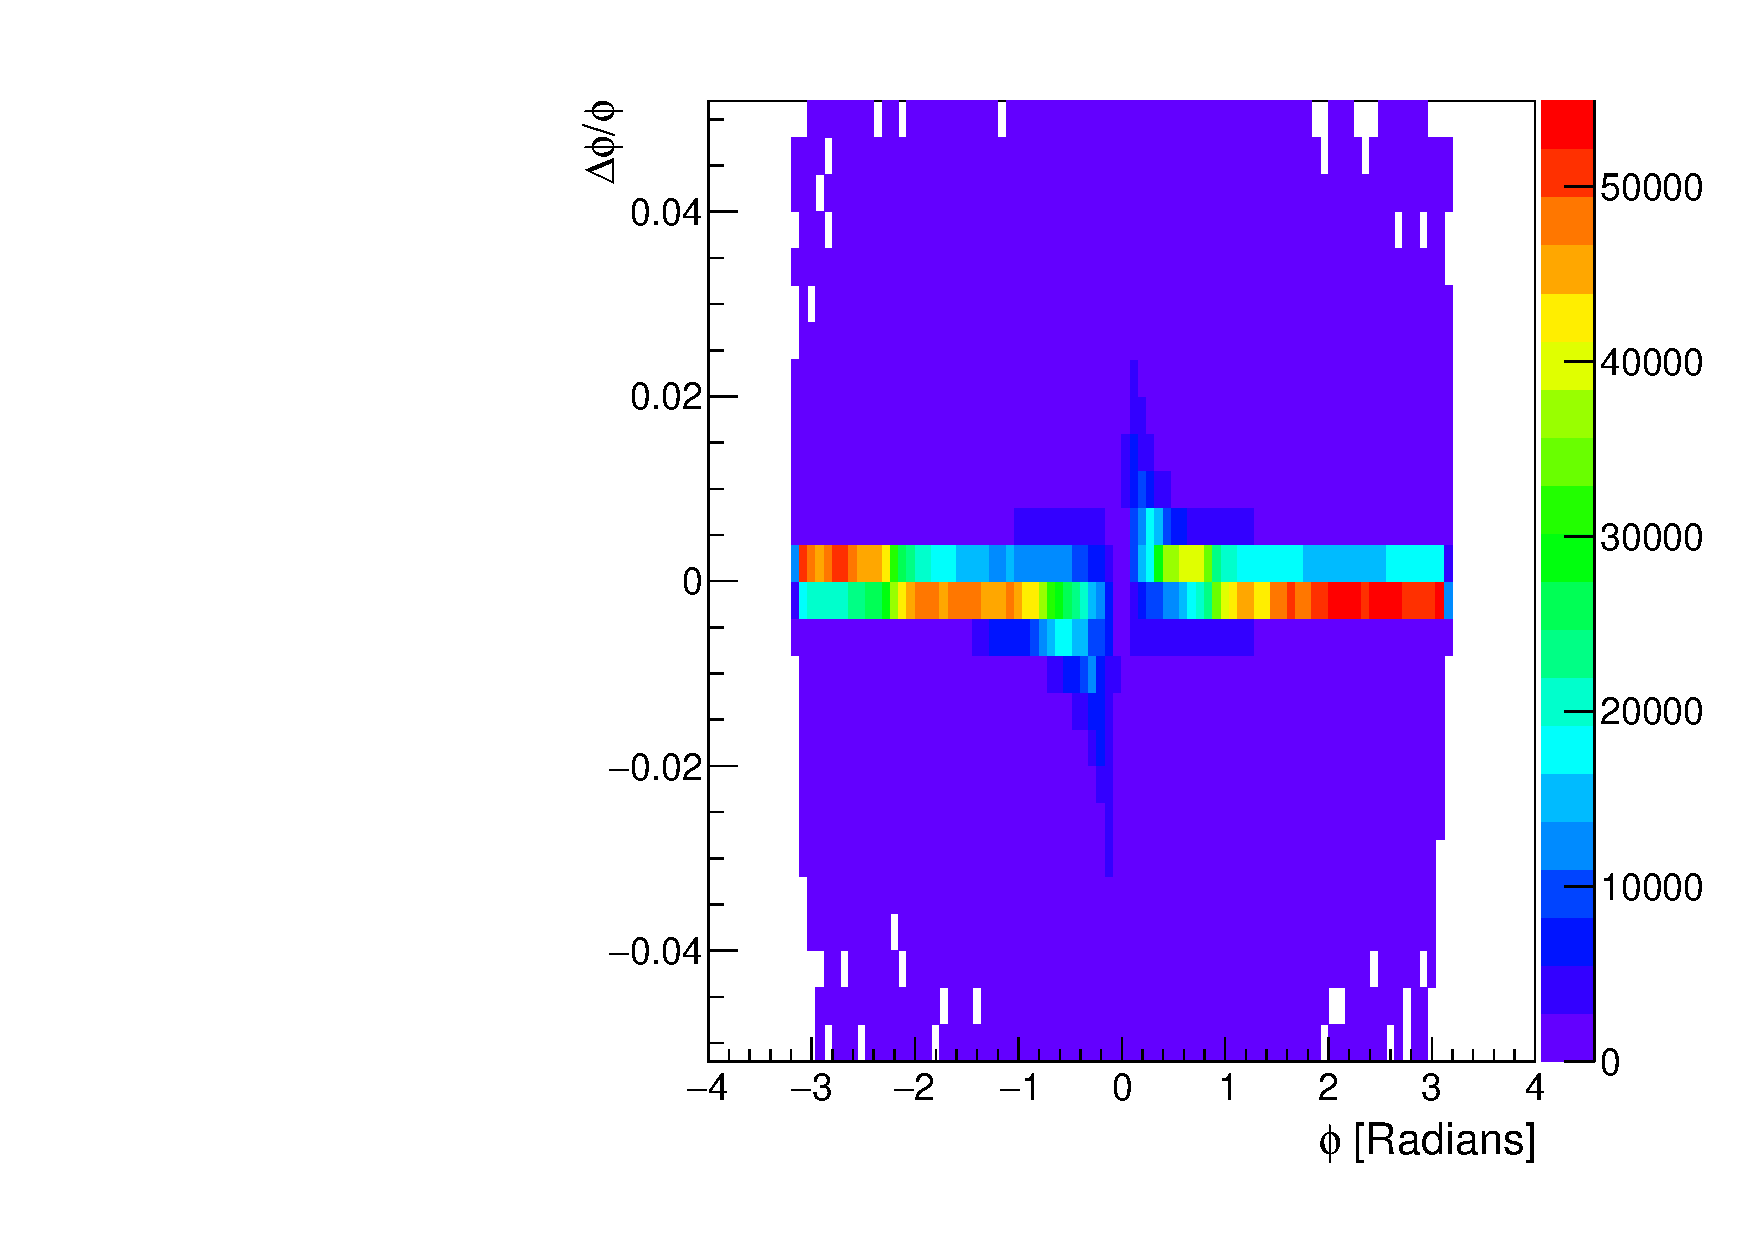
\includegraphics[width=1\linewidth]{Offline_2C_phiRatio_Leading_Non_BJet}
		\end{minipage}
		\caption{$\Delta \phi_{ratio}$ for the leading non \bjet, for Monte-Carlo events (left) and real data (right)}
		\label{fig:O:leadingnonbphi}
	\end{figure}
	
	As with the \bjets, for these other variables offline and online jets produce nearly identical results, with the distribution of $\Delta X_{ratio}$ firmly centred around 0 and a breadth of less than $1\%$.
	
	\subsection{Comparison of Jet Objects between Offline and Online}
		
		The jet objects reconstructed in the HLT have some slight differences in the reported values for key topological variables, but overall they perform in a similar fashion, both in Monte-Carlo simulations and in Real data. The positional variables, $\phi$ and $\eta$ are directly comparable between offline and online jet objects, with the majority of objects having values with $<1\%$ disagreement for both \bjets and non \bjets. For the \pt of jet objects, the values are not in perfect agreement, but have a consistent offset observed in Monte-Carlo and Real data which could be overcome with specific calibration of the jet objects reconstructed in the HLT. 
	
\newpage
\section{Jet Tagging Efficiency}

	As covered in \ref{det:btag:mv}, the standard algorithm for 2016 physics analyses was chosen to be the 2016 MV2c10 algorithm. However, the HLT \btag algorithm uses the MV2c20 algorithm. \cite{trig2015} To perform a valid TLA the perfomance of the tagging algorithms between trigger level and offline must be similar. With the datasets used for this analysis (\ref{dataset}) the MC data produced in 2015 would make use of the older configurations compared to the newer configurations in the data. \note{not sure what effect this config changes had on the trigger}

	Here the tagging efficiency of the HLT and offline taggers is studied for different jet flavours in the MC sample. An offline/HLT jet pair was formed using $\Delta R$ matching and truth label of the jet used to assign a flavour. The efficiency plots in figures \ref{fig:MC:bjetefficiency}, \ref{fig:MC:cjetefficiency} and \ref{fig:MC:lightjetefficiency} show the fraction of these jets that were identified as \bjets by the HLT and offline tagging algorithms.
	
	The jet objects reconstructed online and offline contain the \btagging decision for that object. In the Monte-Carlo xAOD data, the truth label of a jet could be used to determine the exact nature of the jet. The \btagging decision of jets truth labelled as \bjets, \cjets and light-jets was studied for both offline and online to compare the efficiency of the algorithms. 

	\subsection{\textit{b}-jet efficiency}
	
	For jets labelled as true \bjets, the tagging efficiency can be calculated and plotted with respect to topological variables of the jet objects.

		\begin{figure}[h]
			\centering
			\begin{minipage}[h]{0.45\linewidth}
				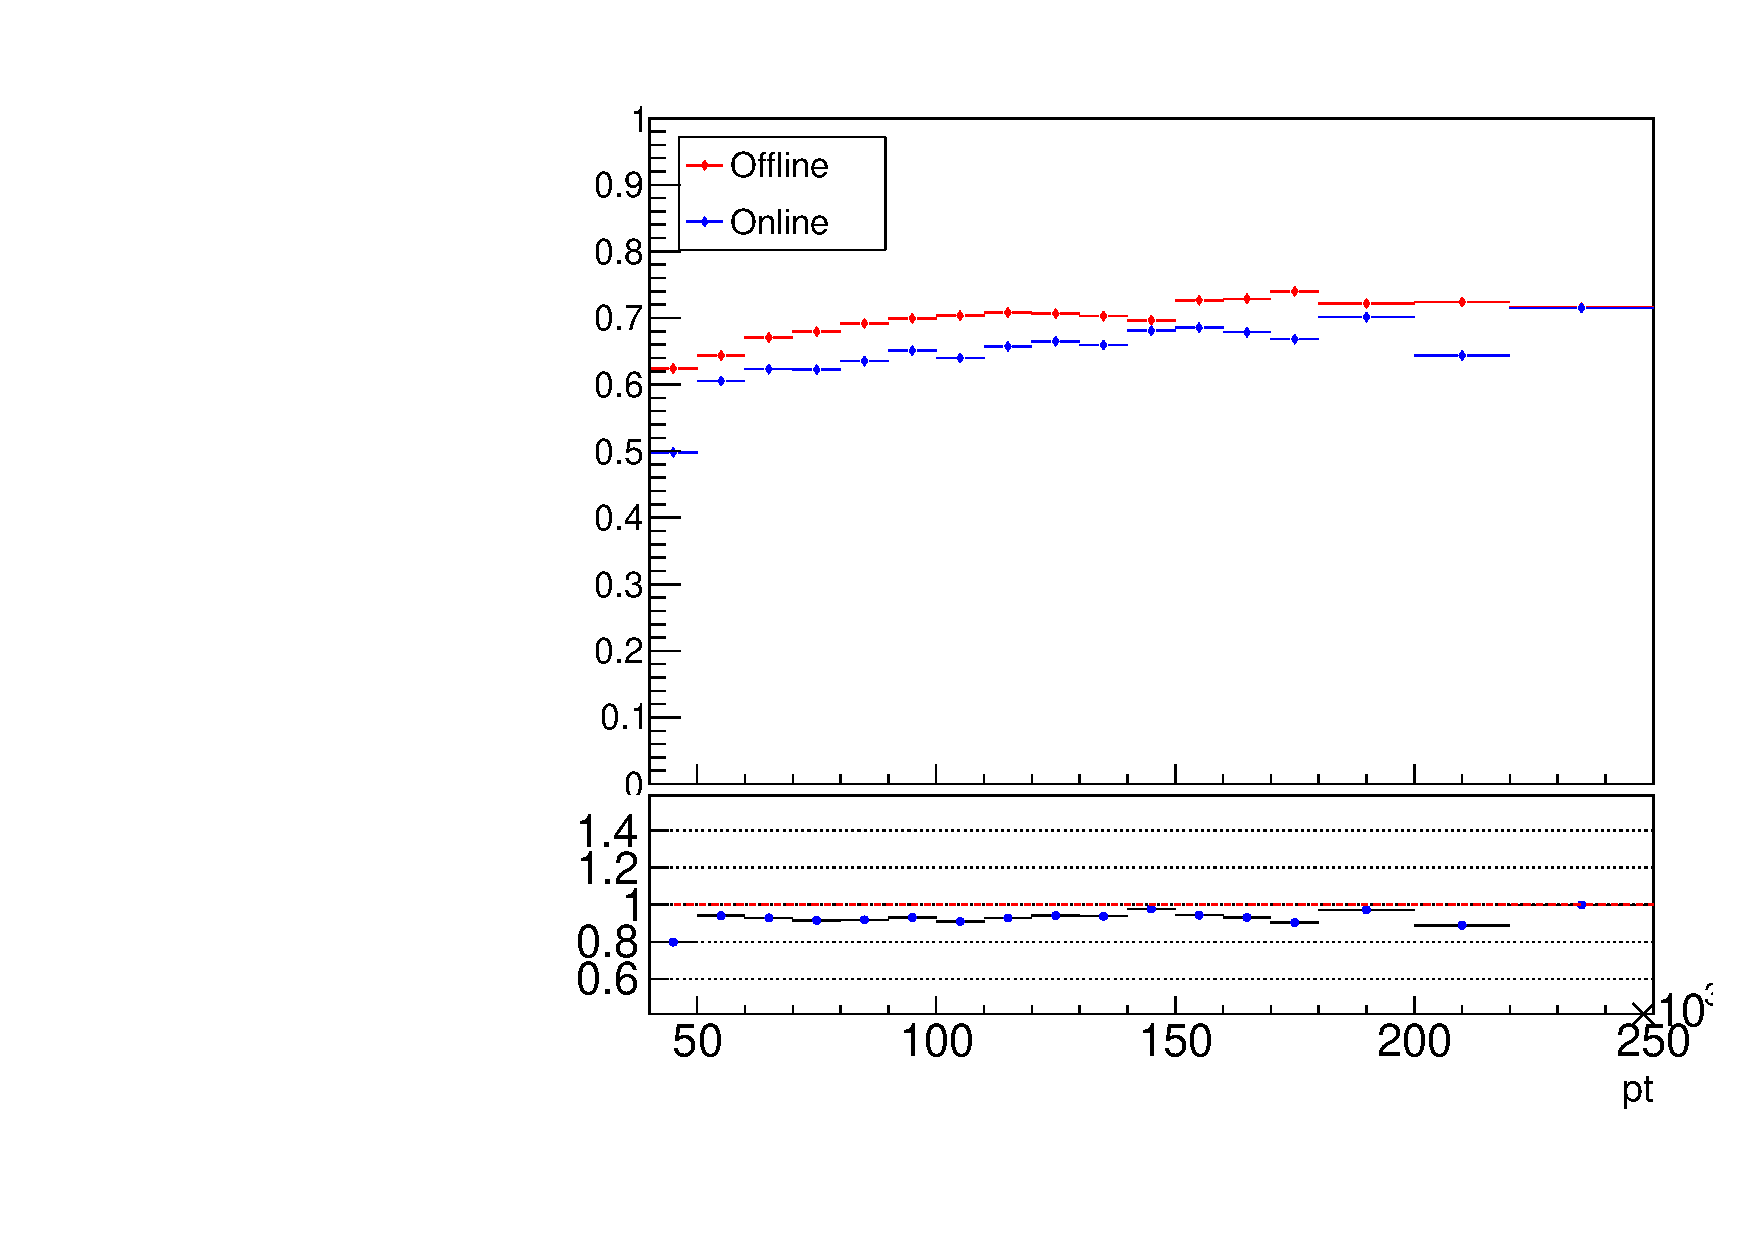
\includegraphics[width=1\linewidth]{ptBJET}

			\end{minipage}
			\quad
			\begin{minipage}[h]{0.45\linewidth}
				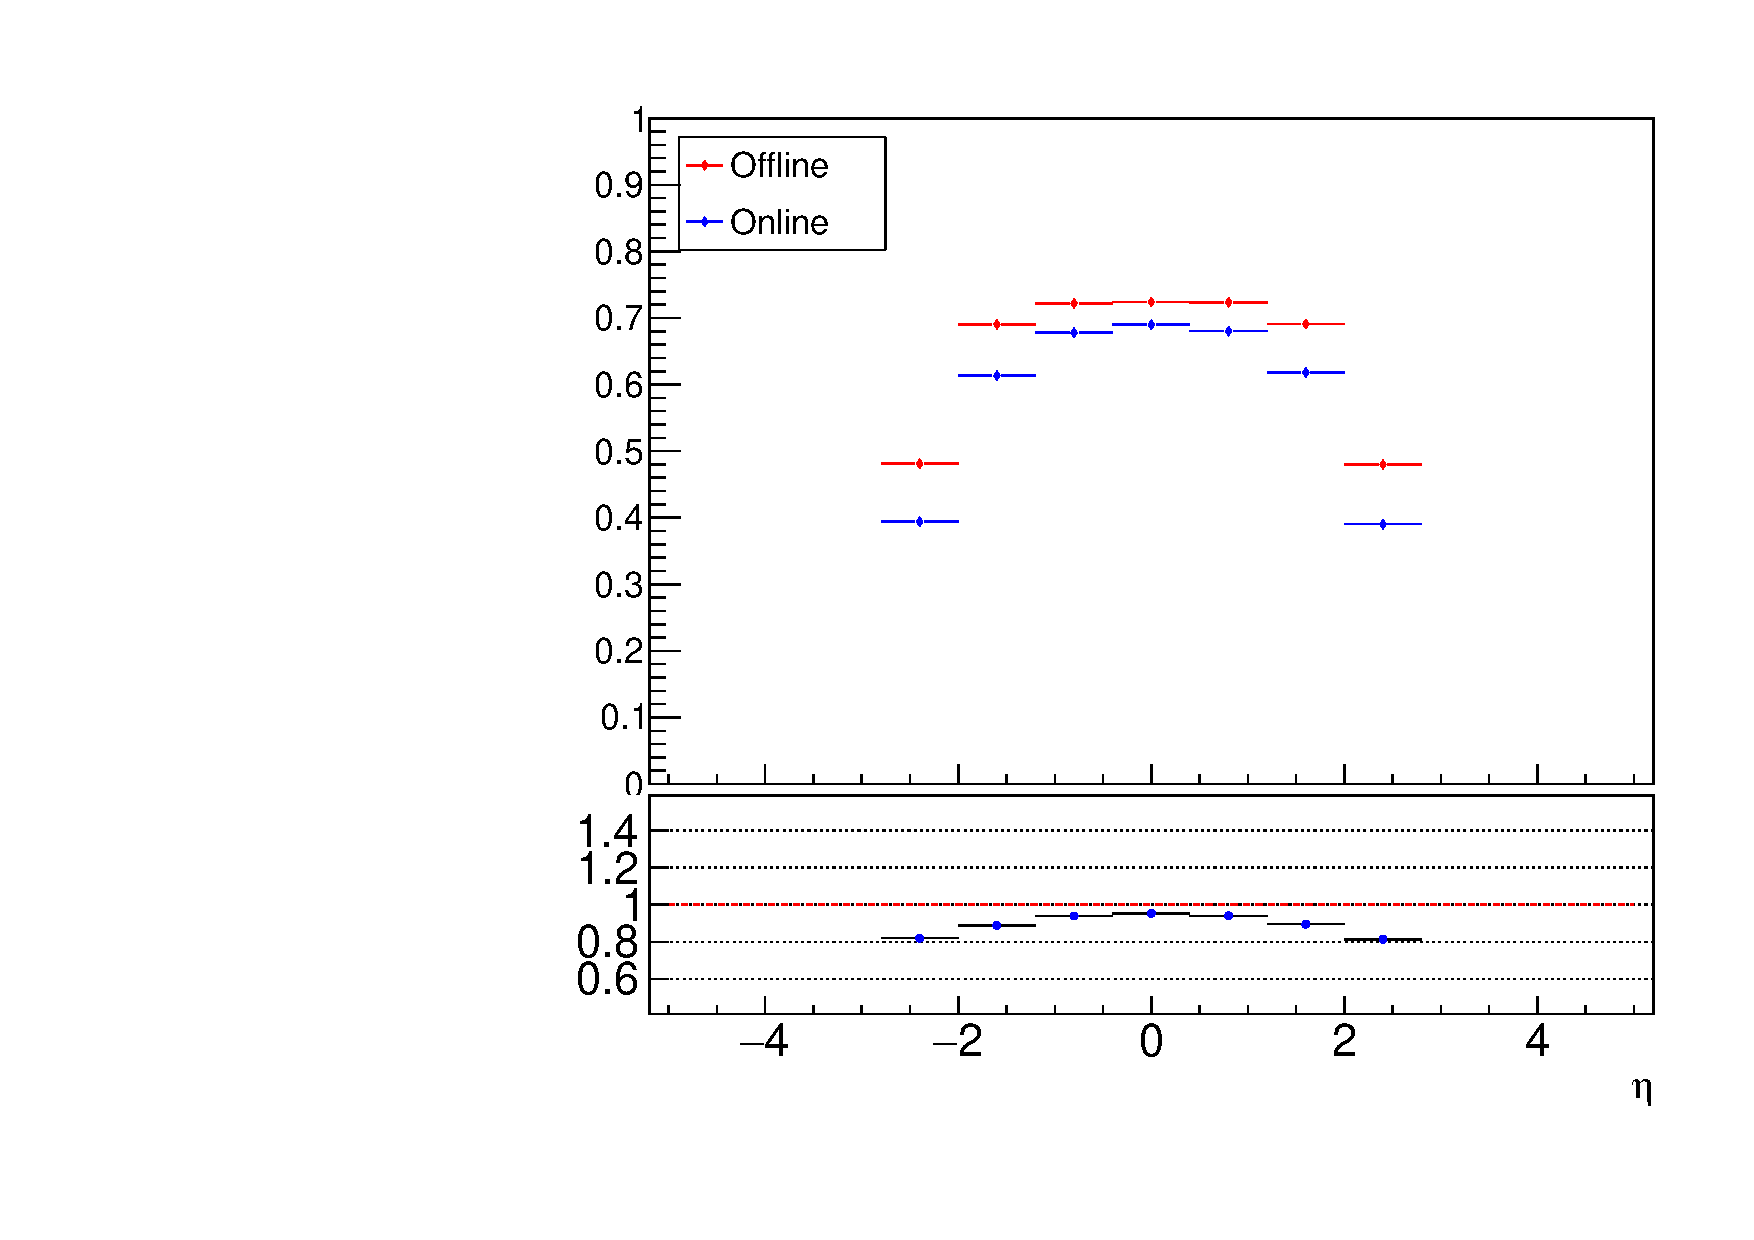
\includegraphics[width=1\linewidth]{etaBJET}
			\end{minipage}
			\caption{\btagging efficiency for truth \bjets in Monte-Carlo data, plotted against jet \pt (left) and $\eta$ (right). Analysis is confined to the central region of the detector where \btagging is operational.}
			\label{fig:MC:bjetefficiency}
		\end{figure}

			\todo{Options, could show more vars or alternatively the reference hists, or alternatively just reference the references}

	\subsection{\textit{c}-jet efficiency}
	
	For \cjets and light-jets, plotting the same value gives the mistag rate for these jets in the detector. 

		\begin{figure}[h]
			\centering
			\begin{minipage}[h]{0.45\linewidth}
				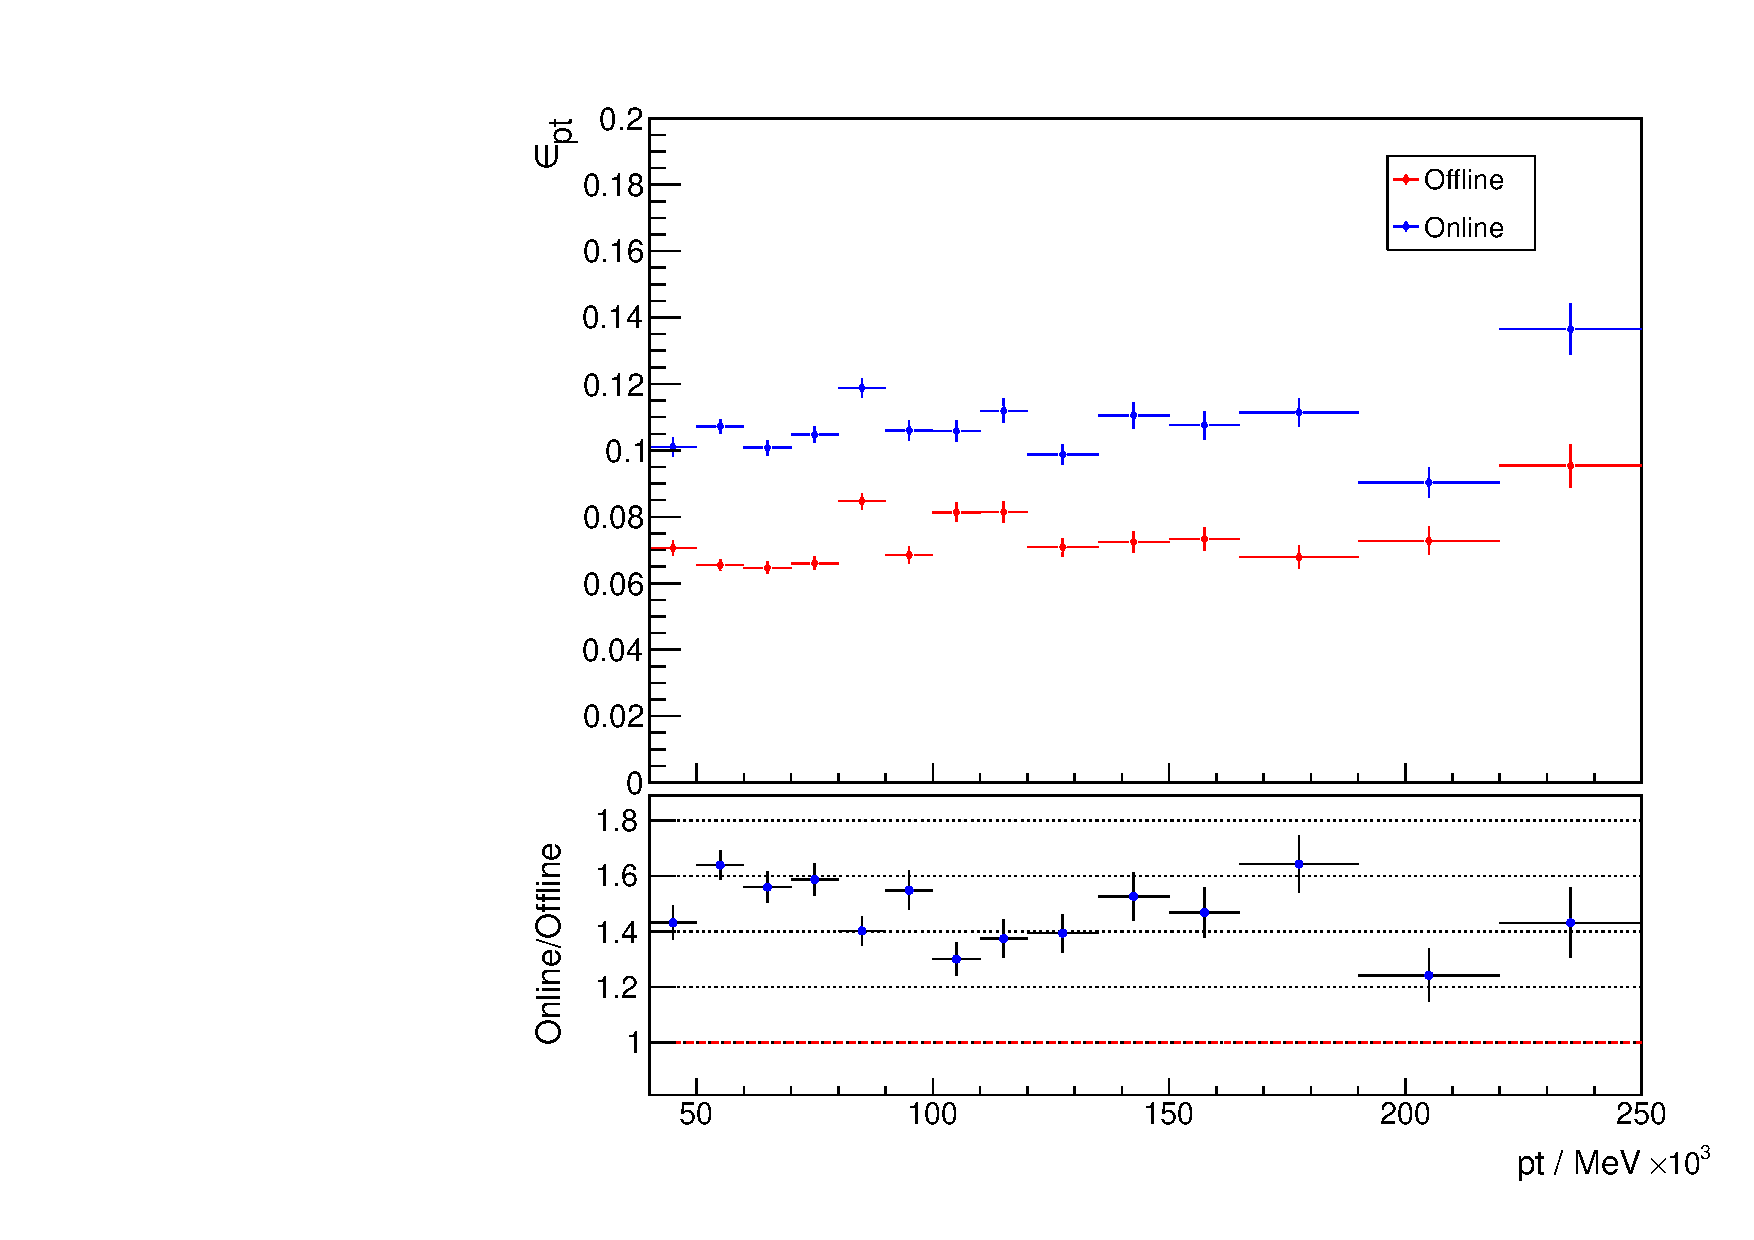
\includegraphics[width=1\linewidth]{ptCJET}

			\end{minipage}
			\quad
			\begin{minipage}[h]{0.45\linewidth}
				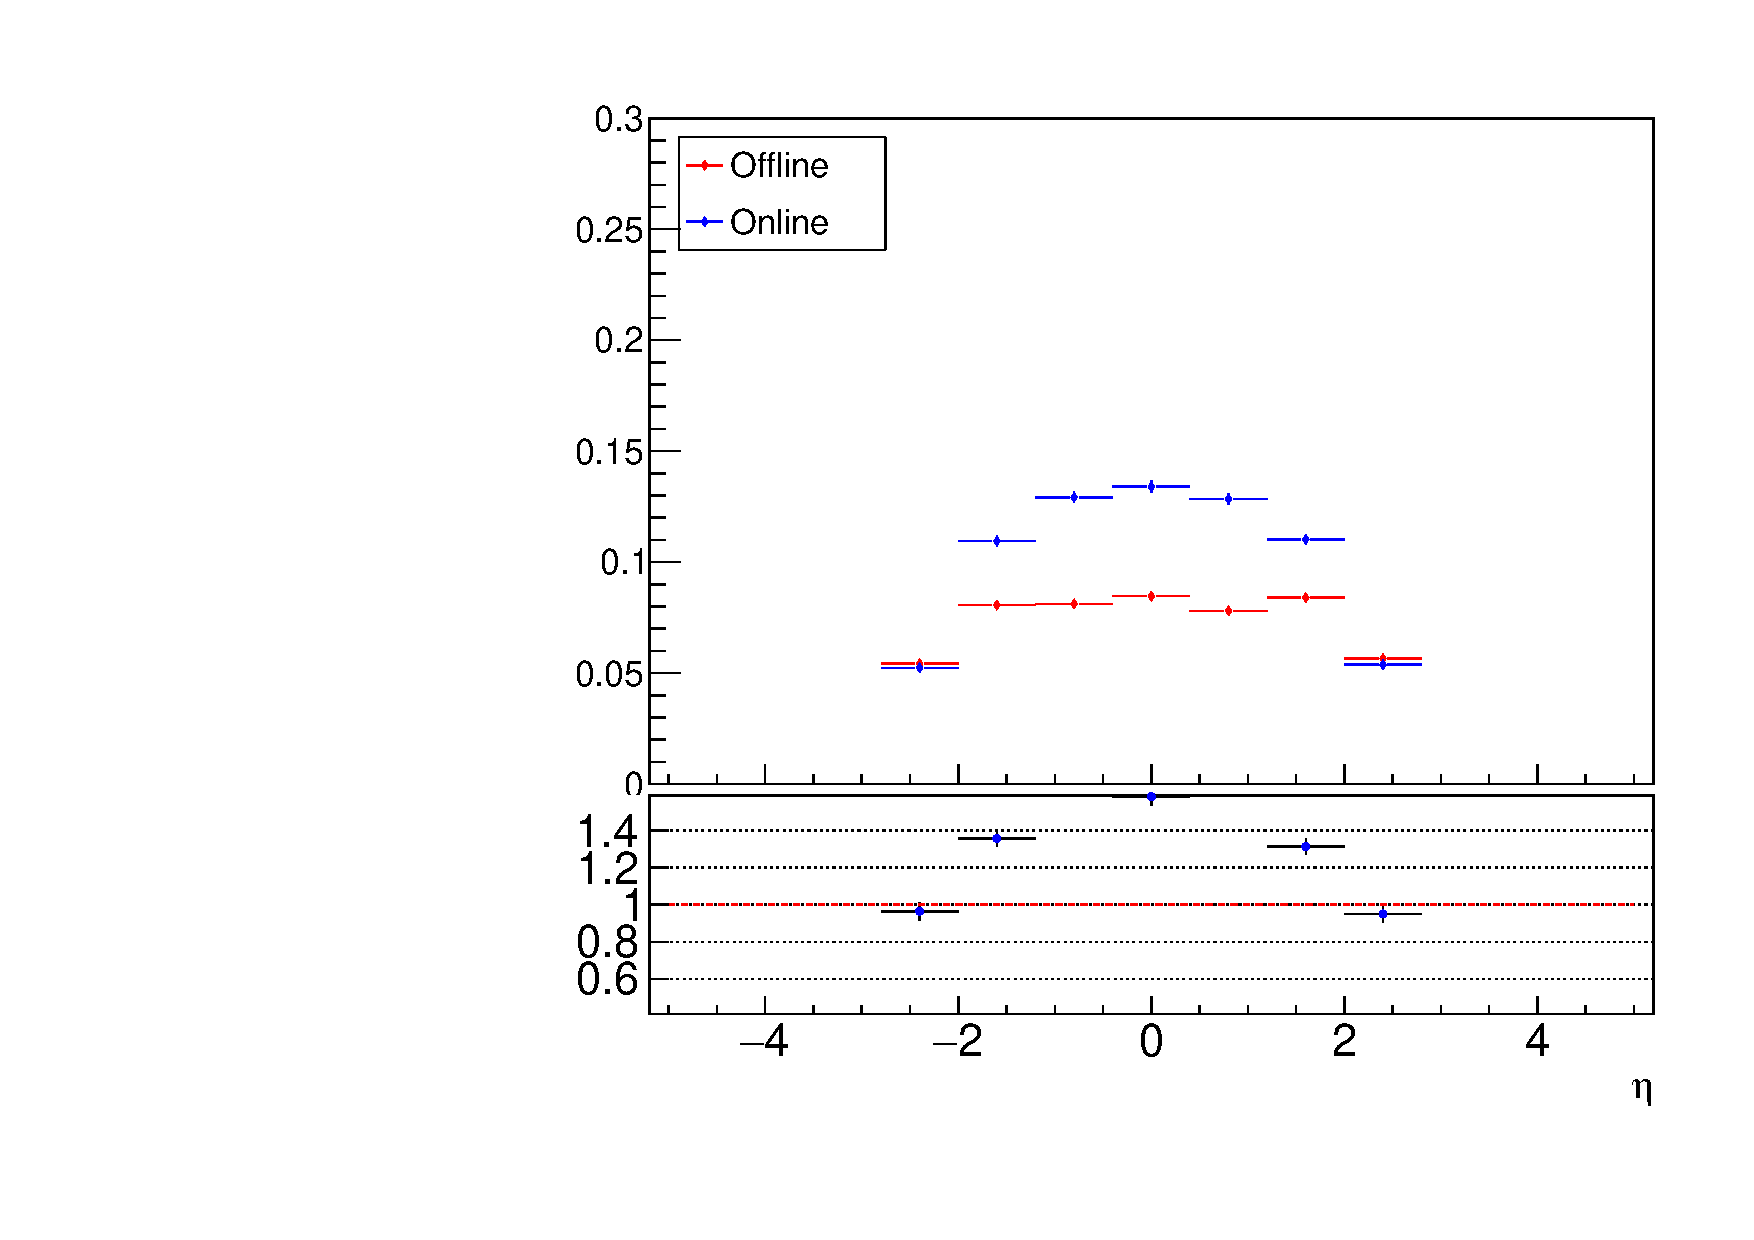
\includegraphics[width=1\linewidth]{etaCJET}
			\end{minipage}
			\caption{Mistag rate for truth \bjets in Monte-Carlo data, plotted against jet \pt (left) and $\eta$ (right). Analysis is confined to the central region of the detector where \btagging is operational.}
			\label{fig:MC:cjetefficiency}
		\end{figure}

	\subsection{Light-jet efficiency}

		\begin{figure}[h]
			\centering
			\begin{minipage}[h]{0.45\linewidth}
				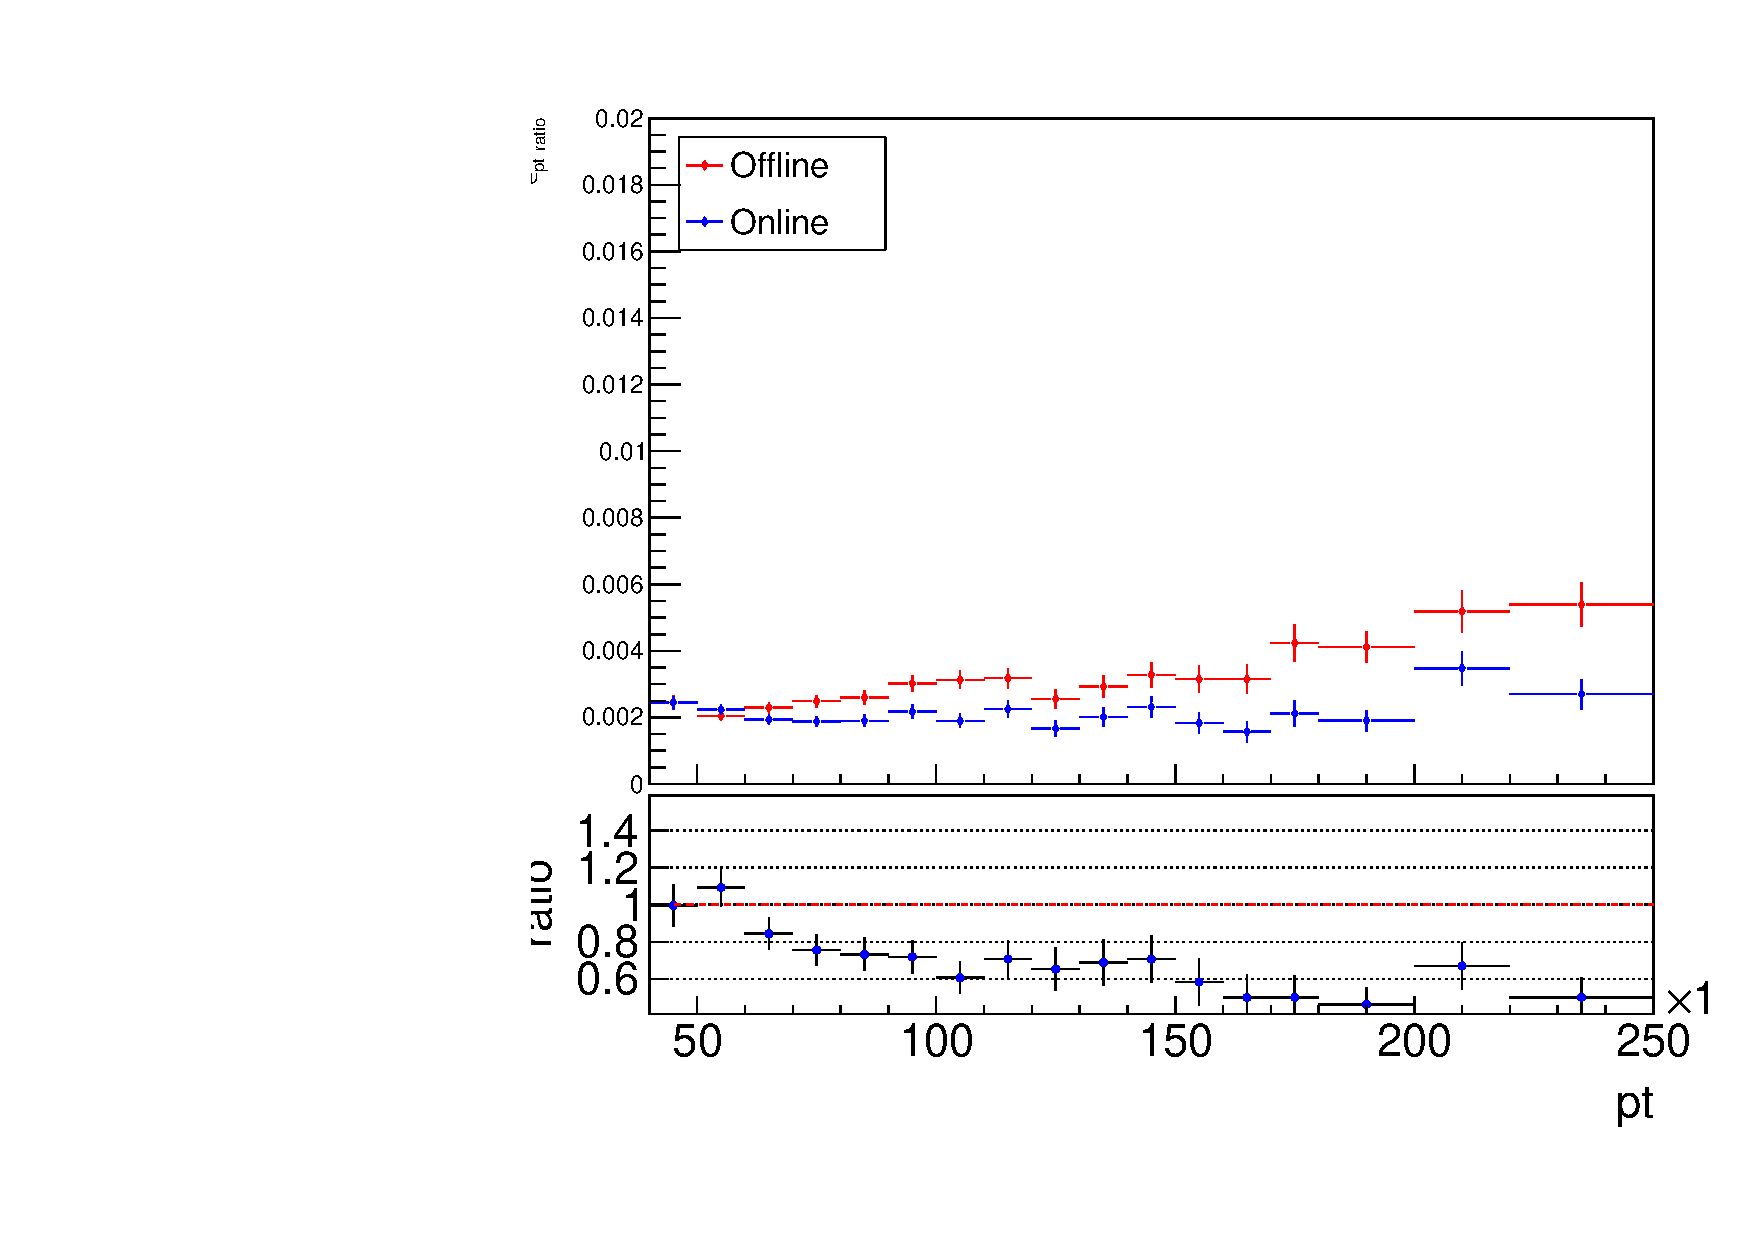
\includegraphics[width=1\linewidth]{ptLIGHTJET}

			\end{minipage}
			\quad
			\begin{minipage}[h]{0.45\linewidth}
				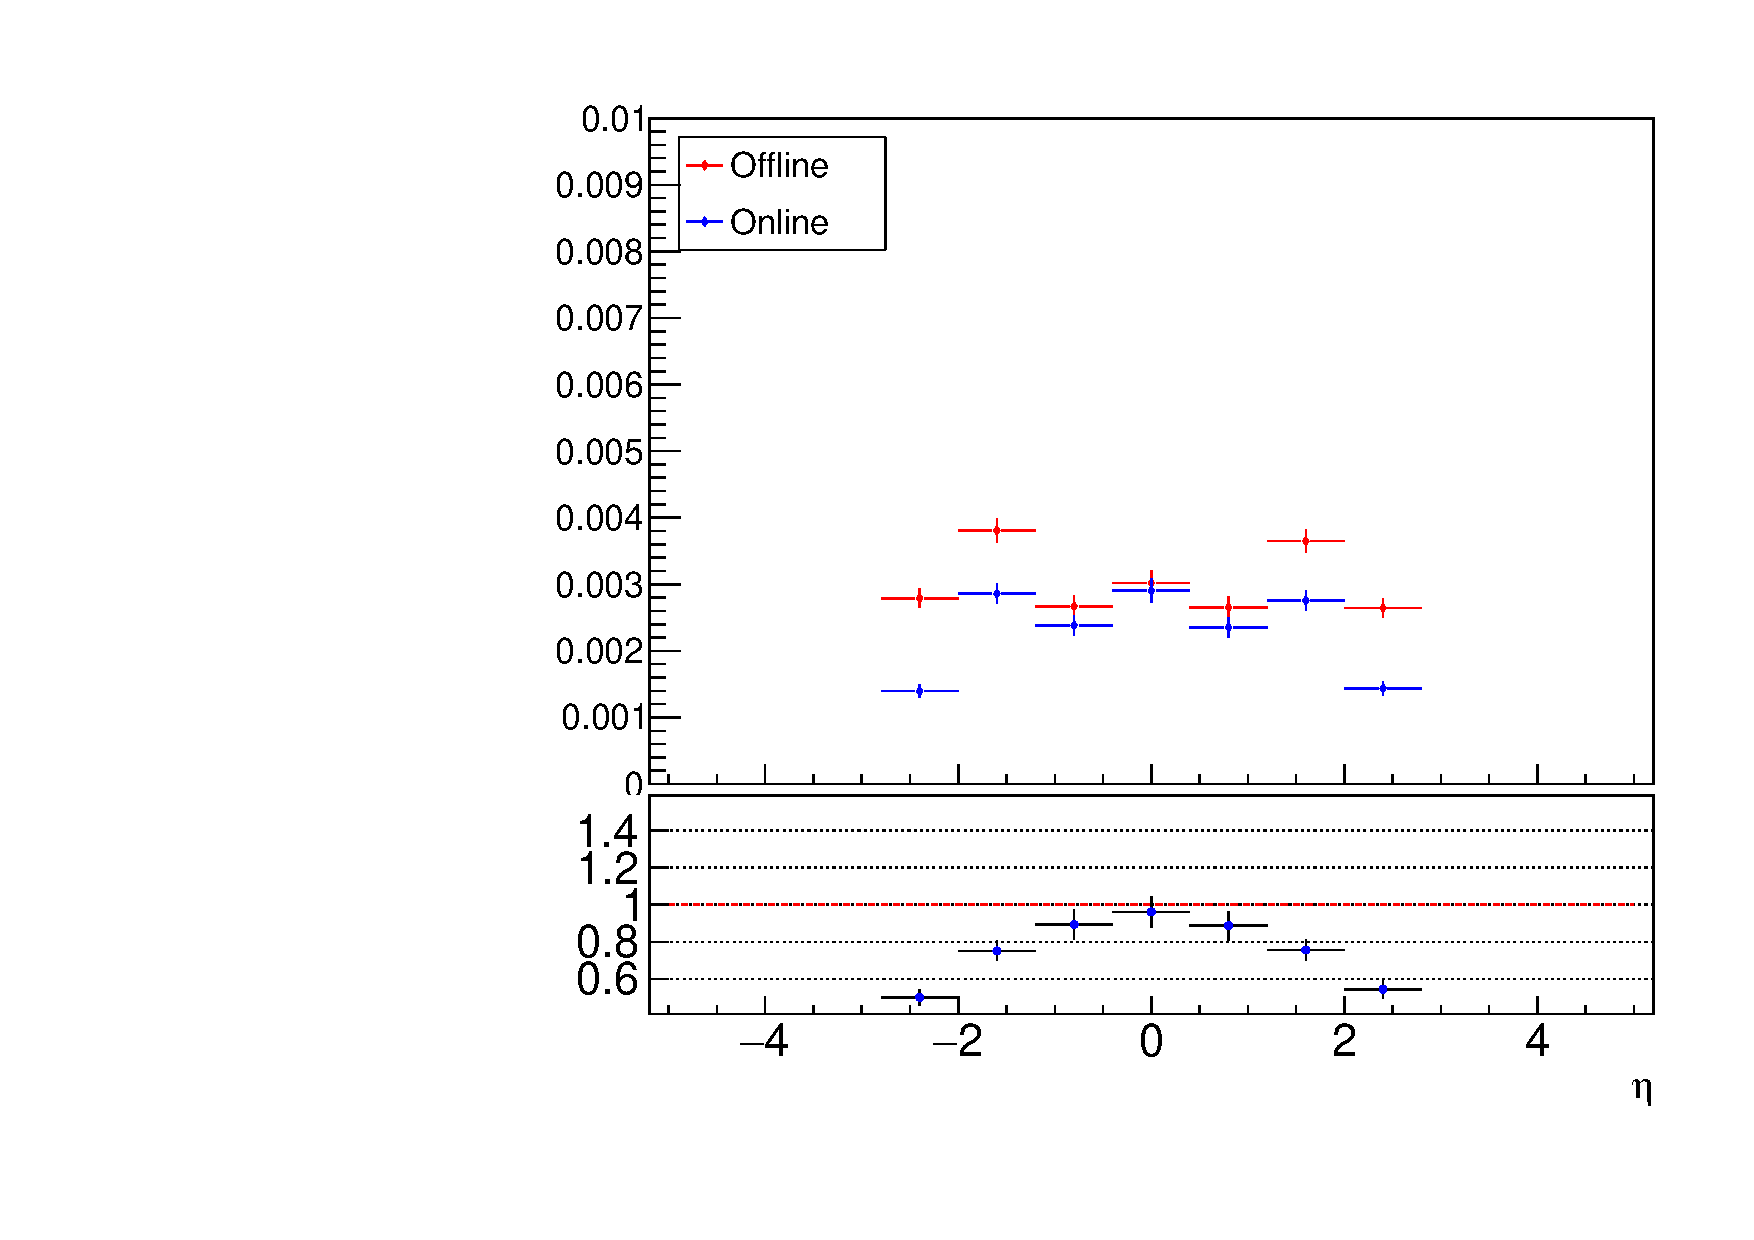
\includegraphics[width=1\linewidth]{etaLIGHTJET}
			\end{minipage}
			\caption{Mistag rate for truth light-jets in Monte-Carlo data, plotted against jet \pt (left) and $\eta$ (right). Analysis is confined to the central region of the detector where \btagging is operational.}
			\label{fig:MC:lightjetefficiency}
		\end{figure}


	\subsection{Tag Matching}

	For each pair of jets that could be matched between online and offline, and then successfully have a $b$-tagging decision evaluated on the jets, the agreement of the $b$-tagging between the two jets was checked. These were found to match one another in $90.91\%$ of cases.

	\subsection{Comparison of HLT and offline tagging efficiencies}

		Primarily considering the \pt plots of efficiency, the HLT \btag is found to be around 5\% less efficient than the offline \btag for jets with \pt$>50$GeV. This is a consistent direction of efficiency shift as found when comparing the 2016 MV2c10 and 2015 MV2c20 algorithms on the training $t\bar{t}$ sample, but of a larger magnitude. The increase in the rate of \cjet mistagging is absolutely consitent with the refinements to the algorithm between the 2016 MV2c10 and 2015 MV2c20, with increased levels of \cjet rejection in the offline 2016 MV2c10, and the $\sim40$\% increase is consistent with the expected shift from the optimised algorithm. \cite{btagOptimisation} The light-jet behaviour is also similar as expected but ????. \todo{some light jet related shenanigans}


	\section{MV2 Discriminant Values - ???} \todo{Necessary}

	\note{Here would show plots of the MV2 value against pt/eta or whatever}



\endinput
